%%%%%%%%%%%%%%%%%%%%%%%%%%%%%%%%%%%%%%%%%%%%%%%%%%%%%%%%%%%%%%%%
% MUW Presentation
% LaTeX Template
% Version 1.0 (27/12/2016)
%
% License:
% CC BY-NC-SA 4.0 (http://creativecommons.org/licenses/by-nc-sa/3.0/)
%
% Created by:
% Nicolas Ballarini, CeMSIIS, Medical University of Vienna
% nicoballarini@gmail.com
% http://statistics.msi.meduniwien.ac.at/
%
% Customized for UAH by:
% David F. Barrero, Departamento de Automática, UAH
%%%%%%%%%%%%%%%%%%%%%%%%%%%%%%%%%%%%%%%%%%%%%%%%%%%%%%%%%%%%%%%%%

\documentclass[10pt,compress]{beamer} % Change 10pt to make fonts of a different size
\mode<presentation>

\usepackage[spanish]{babel}
\usepackage{fontspec}
\usepackage{tikz}
\usepackage{etoolbox}
\usepackage{xcolor}
\usepackage{xstring}
\usepackage{listings}

% Custom packages
\usepackage{multicol}
\usepackage{tikz}
\usepackage{pgfplots}
\def\layersep{2.5cm}
\usetikzlibrary{matrix,chains,positioning,decorations.pathreplacing,arrows}

\definecolor{dkgreen}{rgb}{0,0.6,0}
\definecolor{gray}{rgb}{0.5,0.5,0.5}
\definecolor{mauve}{rgb}{0.58,0,0.82}
 

\usetheme{UAH}
\usecolortheme{UAH}
\setbeamertemplate{navigation symbols}{} 
\setbeamertemplate{caption}[numbered]

%%%%%%%%%%%%%%%%%%%%%%%%%%%%%%%%%%%%%%%%%%%%%%%%%%%%%%%%%%%%%%%%%
%% Presentation Info
\title[Search]{Search}
\author{\asignatura\\\carrera}
\institute{}
\date{Departamento de Automática}
%%%%%%%%%%%%%%%%%%%%%%%%%%%%%%%%%%%%%%%%%%%%%%%%%%%%%%%%%%%%%%%%%


%%%%%%%%%%%%%%%%%%%%%%%%%%%%%%%%%%%%%%%%%%%%%%%%%%%%%%%%%%%%%%%%%
%% Descomentar para habilitar barra de navegación superior
\setNavigation
%%%%%%%%%%%%%%%%%%%%%%%%%%%%%%%%%%%%%%%%%%%%%%%%%%%%%%%%%%%%%%%%%

%%%%%%%%%%%%%%%%%%%%%%%%%%%%%%%%%%%%%%%%%%%%%%%%%%%%%%%%%%%%%%%%%
%% Configuración de logotipos en portada
%% Opacidad de los logotipos
\newcommand{\opacidad}{1}
%% Descomentar para habilitar logotipo en pié de página de portada
\renewcommand{\logoUno}{Images/isg.png}
%% Descomentar para habilitar logotipo en pié de página de portada
%\renewcommand{\logoDos}{Images/CCLogo.png}
%% Descomentar para habilitar logotipo en pié de página de portada
%\renewcommand{\logoTres}{Images/ALogo.png}
%% Descomentar para habilitar logotipo en pié de página de portada
%\renewcommand{\logoCuatro}{Images/ELogo.png}
%%%%%%%%%%%%%%%%%%%%%%%%%%%%%%%%%%%%%%%%%%%%%%%%%%%%%%%%%%%%%%%%%

%%%%%%%%%%%%%%%%%%%%%%%%%%%%%%%%%%%%%%%%%%%%%%%%%%%%%%%%%%%%%%%%%
%% FOOTLINE
%% Comment/Uncomment the following blocks to modify the footline
%% content in the body slides. 


%% Option A: Title and institute
\footlineA
%% Option B: Author and institute
%\footlineB
%% Option C: Title, Author and institute
%\footlineC
%%%%%%%%%%%%%%%%%%%%%%%%%%%%%%%%%%%%%%%%%%%%%%%%%%%%%%%%%%%%%%%%%

\begin{document}

%%%%%%%%%%%%%%%%%%%%%%%%%%%%%%%%%%%%%%%%%%%%%%%%%%%%%%%%%%%%%%%%%
% Use this block for a blue title slide with modified footline
{\titlepageBlue
    \begin{frame}
        \titlepage
    \end{frame}
}

\institute{\asignatura}

\begin{frame}[plain]{}
   \begin{block}{Objectives}
      \begin{enumerate}
         \item Understand the role of search in AI
         \item Describe the importance of trees in search
         \item Express AI problems in terms of search
         \item Apply classical search algorithms (uninformed, informed and local)
      \end{enumerate} 
   \end{block}

   \begin{block}{Bibliography}
	\begin{itemize}
        \item S. Russell and P. Norvig. Chapter 3, Solving Problems by Searching. \textit{Artificial Intelligence: A Modern Approach}. Pearson. 2017
        \item S. Russell and P. Norvig. Chapter 4, Beyond Classical Search. \textit{Artificial Intelligence: A Modern Approach}. Pearson. 2017
	\end{itemize}
   \end{block}
\end{frame}

{
\disableNavigation{white}
\begin{frame}[shrink]{Table of Contents}
 \frametitle{Table of Contents}
    \begin{multicols}{2}
    \tableofcontents
    \end{multicols}
  % You might wish to add the option [pausesections]
\end{frame}
}

\section{Introduction}

\begin{frame}{Introduction}{Intelligent agent}
    \begin{columns}
 	   \column{.50\textwidth}
        \begin{block}{Agent}
        An agent is anything that can be viewed as perceiving its environment through sensors and acting through actuators
        \end{block}

 	   \column{.50\textwidth}
       \begin{center}
	        \includegraphics[width=0.9\linewidth]{figs/agent-environment.eps}\\
	        \tiny{\href{http://aima.cs.berkeley.edu/index.html}{(Source)}}
	    \end{center}

	\end{columns}

    \begin{itemize}
        \item Agents is a research field in AI by its own 
            \begin{itemize}
                \item ... with its own definition of agent (caution!)
            \end{itemize}
        \item We use this term to abstract the implementation
    \end{itemize}
\end{frame}

\begin{frame}{Introduction}{Motivation}

    \begin{columns}
 	   \column{.60\textwidth}

    Early AI works were directed to
    \begin{itemize}
        \item Proof of theorems, crosswords, games, ...
    \end{itemize}

    All in AI is search ...
    \begin{itemize}
        \item ... not entirely true (obviously) but more than we may imagine
        \item Find a good/best solution (\alert{solution space}) to a problem among several potential solutions (\alert{search space})
    \end{itemize}

    \textbf{Enhaustive search} (or brute-force search)
    \begin{itemize}
        \item Iterate over all the potential solutions
        \item Unsuiteable for most real-world problems
    \end{itemize}

 	\column{.40\textwidth}
     %rch
%%%%%%%%%%%%%%%%%%%%%%%%%%%%%%%%%%%%%%%%%%%%%%%%%%%%%%%%%%%%%%%%
% MUW Presentation
% LaTeX Template
% Version 1.0 (27/12/2016)
%
% License:
% CC BY-NC-SA 4.0 (http://creativecommons.org/licenses/by-nc-sa/3.0/)
%
% Created by:
% Nicolas Ballarini, CeMSIIS, Medical University of Vienna
% nicoballarini@gmail.com
% http://statistics.msi.meduniwien.ac.at/
%
% Customized for UAH by:
% David F. Barrero, Departamento de Automática, UAH
%%%%%%%%%%%%%%%%%%%%%%%%%%%%%%%%%%%%%%%%%%%%%%%%%%%%%%%%%%%%%%%%%

\documentclass[10pt,compress]{beamer} % Change 10pt to make fonts of a different size
\mode<presentation>

\usepackage[spanish]{babel}
\usepackage{fontspec}
\usepackage{tikz}
\usepackage{etoolbox}
\usepackage{xcolor}
\usepackage{xstring}
\usepackage{listings}

% Custom packages
\usepackage{tikz}
\usepackage{pgfplots}
\def\layersep{2.5cm}
\usetikzlibrary{matrix,chains,positioning,decorations.pathreplacing,arrows}

\definecolor{dkgreen}{rgb}{0,0.6,0}
\definecolor{gray}{rgb}{0.5,0.5,0.5}
\definecolor{mauve}{rgb}{0.58,0,0.82}
 

\usetheme{UAH}
\usecolortheme{UAH}
\setbeamertemplate{navigation symbols}{} 
\setbeamertemplate{caption}[numbered]

%%%%%%%%%%%%%%%%%%%%%%%%%%%%%%%%%%%%%%%%%%%%%%%%%%%%%%%%%%%%%%%%%
%% Presentation Info
\title[Search algorithm]{Solving Problems by Searching}
\author{\asignatura\\\carrera}
\institute{}
\date{Departamento de Automática}
%%%%%%%%%%%%%%%%%%%%%%%%%%%%%%%%%%%%%%%%%%%%%%%%%%%%%%%%%%%%%%%%%


%%%%%%%%%%%%%%%%%%%%%%%%%%%%%%%%%%%%%%%%%%%%%%%%%%%%%%%%%%%%%%%%%
%% Descomentar para habilitar barra de navegación superior
\setNavigation
%%%%%%%%%%%%%%%%%%%%%%%%%%%%%%%%%%%%%%%%%%%%%%%%%%%%%%%%%%%%%%%%%

%%%%%%%%%%%%%%%%%%%%%%%%%%%%%%%%%%%%%%%%%%%%%%%%%%%%%%%%%%%%%%%%%
%% Configuración de logotipos en portada
%% Opacidad de los logotipos
\newcommand{\opacidad}{1}
%% Descomentar para habilitar logotipo en pié de página de portada
\renewcommand{\logoUno}{Images/isg.png}
%% Descomentar para habilitar logotipo en pié de página de portada
%\renewcommand{\logoDos}{Images/CCLogo.png}
%% Descomentar para habilitar logotipo en pié de página de portada
%\renewcommand{\logoTres}{Images/ALogo.png}
%% Descomentar para habilitar logotipo en pié de página de portada
%\renewcommand{\logoCuatro}{Images/ELogo.png}
%%%%%%%%%%%%%%%%%%%%%%%%%%%%%%%%%%%%%%%%%%%%%%%%%%%%%%%%%%%%%%%%%

%%%%%%%%%%%%%%%%%%%%%%%%%%%%%%%%%%%%%%%%%%%%%%%%%%%%%%%%%%%%%%%%%
%% FOOTLINE
%% Comment/Uncomment the following blocks to modify the footline
%% content in the body slides. 


%% Option A: Title and institute
\footlineA
%% Option B: Author and institute
%\footlineB
%% Option C: Title, Author and institute
%\footlineC
%%%%%%%%%%%%%%%%%%%%%%%%%%%%%%%%%%%%%%%%%%%%%%%%%%%%%%%%%%%%%%%%%

\begin{document}

%%%%%%%%%%%%%%%%%%%%%%%%%%%%%%%%%%%%%%%%%%%%%%%%%%%%%%%%%%%%%%%%%
% Use this block for a blue title slide with modified footline
{\titlepageBlue
    \begin{frame}
        \titlepage
    \end{frame}
}

\institute{\asignatura}

\begin{frame}[plain]{}
   \begin{block}{Objectives}
      \begin{enumerate}
         \item Understand the role of search in AI
         \item Describe the importance of trees in search
         \item Express AI problems in terms of search
         \item Apply classical search algorithms
      \end{enumerate} 
   \end{block}

   \begin{block}{Bibliography}
	\begin{itemize}
        \item S. Russell and P. Norvig. Chapter 3, Solving Problems by Searching. \textit{Artificial Intelligence: A Modern Approach}. Pearson. 2017
	\end{itemize}
   \end{block}
\end{frame}

{
\disableNavigation{white}
\begin{frame}[shrink]{Table of Contents}
 \frametitle{Table of Contents}
 \tableofcontents
  % You might wish to add the option [pausesections]
\end{frame}
}

\section{Introduction}

\begin{frame}{Introduction}{Intelligent agent}
    \begin{columns}
 	   \column{.50\textwidth}
        \begin{block}{Agent}
        An agent is anything that can be viewed as perceiving its environment through sensors and acting through actuators
        \end{block}

 	   \column{.50\textwidth}
       \begin{center}
	        \includegraphics[width=0.9\linewidth]{figs/agent-environment.eps}\\
	        \tiny{\href{http://aima.cs.berkeley.edu/index.html}{(Source)}}
	    \end{center}

	\end{columns}

    \begin{itemize}
        \item Agents is a research field in AI by its own 
            \begin{itemize}
                \item ... with its own definition of agent (caution!)
            \end{itemize}
        \item We use this term to abstract the implementation
    \end{itemize}
\end{frame}

\begin{frame}{Introduction}{Motivation}

    \begin{columns}
 	   \column{.60\textwidth}

    Early AI works were directed to
    \begin{itemize}
        \item Proof of theorems, crosswords, games, ...
    \end{itemize}

    All in AI is search ...
    \begin{itemize}
        \item ... not entirely true (obviously) but more than we may imagine
        \item Find a good/best solution (\alert{solution space}) to a problem among several potential solutions (\alert{search space})
    \end{itemize}

    \textbf{Enhaustive search} (or brute-force search)
    \begin{itemize}
        \item Iterate over all the potential solutions
        \item Unsuiteable for most real-world problems
    \end{itemize}

 	\column{.40\textwidth}
     %rch
%%%%%%%%%%%%%%%%%%%%%%%%%%%%%%%%%%%%%%%%%%%%%%%%%%%%%%%%%%%%%%%%
% MUW Presentation
% LaTeX Template
% Version 1.0 (27/12/2016)
%
% License:
% CC BY-NC-SA 4.0 (http://creativecommons.org/licenses/by-nc-sa/3.0/)
%
% Created by:
% Nicolas Ballarini, CeMSIIS, Medical University of Vienna
% nicoballarini@gmail.com
% http://statistics.msi.meduniwien.ac.at/
%
% Customized for UAH by:
% David F. Barrero, Departamento de Automática, UAH
%%%%%%%%%%%%%%%%%%%%%%%%%%%%%%%%%%%%%%%%%%%%%%%%%%%%%%%%%%%%%%%%%

\documentclass[10pt,compress]{beamer} % Change 10pt to make fonts of a different size
\mode<presentation>

\usepackage[spanish]{babel}
\usepackage{fontspec}
\usepackage{tikz}
\usepackage{etoolbox}
\usepackage{xcolor}
\usepackage{xstring}
\usepackage{listings}

% Custom packages
\usepackage{tikz}
\usepackage{pgfplots}
\def\layersep{2.5cm}
\usetikzlibrary{matrix,chains,positioning,decorations.pathreplacing,arrows}

\definecolor{dkgreen}{rgb}{0,0.6,0}
\definecolor{gray}{rgb}{0.5,0.5,0.5}
\definecolor{mauve}{rgb}{0.58,0,0.82}
 

\usetheme{UAH}
\usecolortheme{UAH}
\setbeamertemplate{navigation symbols}{} 
\setbeamertemplate{caption}[numbered]

%%%%%%%%%%%%%%%%%%%%%%%%%%%%%%%%%%%%%%%%%%%%%%%%%%%%%%%%%%%%%%%%%
%% Presentation Info
\title[Search algorithm]{Solving Problems by Searching}
\author{\asignatura\\\carrera}
\institute{}
\date{Departamento de Automática}
%%%%%%%%%%%%%%%%%%%%%%%%%%%%%%%%%%%%%%%%%%%%%%%%%%%%%%%%%%%%%%%%%


%%%%%%%%%%%%%%%%%%%%%%%%%%%%%%%%%%%%%%%%%%%%%%%%%%%%%%%%%%%%%%%%%
%% Descomentar para habilitar barra de navegación superior
\setNavigation
%%%%%%%%%%%%%%%%%%%%%%%%%%%%%%%%%%%%%%%%%%%%%%%%%%%%%%%%%%%%%%%%%

%%%%%%%%%%%%%%%%%%%%%%%%%%%%%%%%%%%%%%%%%%%%%%%%%%%%%%%%%%%%%%%%%
%% Configuración de logotipos en portada
%% Opacidad de los logotipos
\newcommand{\opacidad}{1}
%% Descomentar para habilitar logotipo en pié de página de portada
\renewcommand{\logoUno}{Images/isg.png}
%% Descomentar para habilitar logotipo en pié de página de portada
%\renewcommand{\logoDos}{Images/CCLogo.png}
%% Descomentar para habilitar logotipo en pié de página de portada
%\renewcommand{\logoTres}{Images/ALogo.png}
%% Descomentar para habilitar logotipo en pié de página de portada
%\renewcommand{\logoCuatro}{Images/ELogo.png}
%%%%%%%%%%%%%%%%%%%%%%%%%%%%%%%%%%%%%%%%%%%%%%%%%%%%%%%%%%%%%%%%%

%%%%%%%%%%%%%%%%%%%%%%%%%%%%%%%%%%%%%%%%%%%%%%%%%%%%%%%%%%%%%%%%%
%% FOOTLINE
%% Comment/Uncomment the following blocks to modify the footline
%% content in the body slides. 


%% Option A: Title and institute
\footlineA
%% Option B: Author and institute
%\footlineB
%% Option C: Title, Author and institute
%\footlineC
%%%%%%%%%%%%%%%%%%%%%%%%%%%%%%%%%%%%%%%%%%%%%%%%%%%%%%%%%%%%%%%%%

\begin{document}

%%%%%%%%%%%%%%%%%%%%%%%%%%%%%%%%%%%%%%%%%%%%%%%%%%%%%%%%%%%%%%%%%
% Use this block for a blue title slide with modified footline
{\titlepageBlue
    \begin{frame}
        \titlepage
    \end{frame}
}

\institute{\asignatura}

\begin{frame}[plain]{}
   \begin{block}{Objectives}
      \begin{enumerate}
         \item Understand the role of search in AI
         \item Describe the importance of trees in search
         \item Express AI problems in terms of search
         \item Apply classical search algorithms
      \end{enumerate} 
   \end{block}

   \begin{block}{Bibliography}
	\begin{itemize}
        \item S. Russell and P. Norvig. Chapter 3, Solving Problems by Searching. \textit{Artificial Intelligence: A Modern Approach}. Pearson. 2017
	\end{itemize}
   \end{block}
\end{frame}

{
\disableNavigation{white}
\begin{frame}[shrink]{Table of Contents}
 \frametitle{Table of Contents}
 \tableofcontents
  % You might wish to add the option [pausesections]
\end{frame}
}

\section{Introduction}

\begin{frame}{Introduction}{Intelligent agent}
    \begin{columns}
 	   \column{.50\textwidth}
        \begin{block}{Agent}
        An agent is anything that can be viewed as perceiving its environment through sensors and acting through actuators
        \end{block}

 	   \column{.50\textwidth}
       \begin{center}
	        \includegraphics[width=0.9\linewidth]{figs/agent-environment.eps}\\
	        \tiny{\href{http://aima.cs.berkeley.edu/index.html}{(Source)}}
	    \end{center}

	\end{columns}

    \begin{itemize}
        \item Agents is a research field in AI by its own 
            \begin{itemize}
                \item ... with its own definition of agent (caution!)
            \end{itemize}
        \item We use this term to abstract the implementation
    \end{itemize}
\end{frame}

\begin{frame}{Introduction}{Motivation}

    \begin{columns}
 	   \column{.60\textwidth}

    Early AI works were directed to
    \begin{itemize}
        \item Proof of theorems, crosswords, games, ...
    \end{itemize}

    All in AI is search ...
    \begin{itemize}
        \item ... not entirely true (obviously) but more than we may imagine
        \item Find a good/best solution (\alert{solution space}) to a problem among several potential solutions (\alert{search space})
    \end{itemize}

    \textbf{Enhaustive search} (or brute-force search)
    \begin{itemize}
        \item Iterate over all the potential solutions
        \item Unsuiteable for most real-world problems
    \end{itemize}

 	\column{.40\textwidth}
     %rch
%%%%%%%%%%%%%%%%%%%%%%%%%%%%%%%%%%%%%%%%%%%%%%%%%%%%%%%%%%%%%%%%
% MUW Presentation
% LaTeX Template
% Version 1.0 (27/12/2016)
%
% License:
% CC BY-NC-SA 4.0 (http://creativecommons.org/licenses/by-nc-sa/3.0/)
%
% Created by:
% Nicolas Ballarini, CeMSIIS, Medical University of Vienna
% nicoballarini@gmail.com
% http://statistics.msi.meduniwien.ac.at/
%
% Customized for UAH by:
% David F. Barrero, Departamento de Automática, UAH
%%%%%%%%%%%%%%%%%%%%%%%%%%%%%%%%%%%%%%%%%%%%%%%%%%%%%%%%%%%%%%%%%

\documentclass[10pt,compress]{beamer} % Change 10pt to make fonts of a different size
\mode<presentation>

\usepackage[spanish]{babel}
\usepackage{fontspec}
\usepackage{tikz}
\usepackage{etoolbox}
\usepackage{xcolor}
\usepackage{xstring}
\usepackage{listings}

% Custom packages
\usepackage{tikz}
\usepackage{pgfplots}
\def\layersep{2.5cm}
\usetikzlibrary{matrix,chains,positioning,decorations.pathreplacing,arrows}

\definecolor{dkgreen}{rgb}{0,0.6,0}
\definecolor{gray}{rgb}{0.5,0.5,0.5}
\definecolor{mauve}{rgb}{0.58,0,0.82}
 

\usetheme{UAH}
\usecolortheme{UAH}
\setbeamertemplate{navigation symbols}{} 
\setbeamertemplate{caption}[numbered]

%%%%%%%%%%%%%%%%%%%%%%%%%%%%%%%%%%%%%%%%%%%%%%%%%%%%%%%%%%%%%%%%%
%% Presentation Info
\title[Search algorithm]{Solving Problems by Searching}
\author{\asignatura\\\carrera}
\institute{}
\date{Departamento de Automática}
%%%%%%%%%%%%%%%%%%%%%%%%%%%%%%%%%%%%%%%%%%%%%%%%%%%%%%%%%%%%%%%%%


%%%%%%%%%%%%%%%%%%%%%%%%%%%%%%%%%%%%%%%%%%%%%%%%%%%%%%%%%%%%%%%%%
%% Descomentar para habilitar barra de navegación superior
\setNavigation
%%%%%%%%%%%%%%%%%%%%%%%%%%%%%%%%%%%%%%%%%%%%%%%%%%%%%%%%%%%%%%%%%

%%%%%%%%%%%%%%%%%%%%%%%%%%%%%%%%%%%%%%%%%%%%%%%%%%%%%%%%%%%%%%%%%
%% Configuración de logotipos en portada
%% Opacidad de los logotipos
\newcommand{\opacidad}{1}
%% Descomentar para habilitar logotipo en pié de página de portada
\renewcommand{\logoUno}{Images/isg.png}
%% Descomentar para habilitar logotipo en pié de página de portada
%\renewcommand{\logoDos}{Images/CCLogo.png}
%% Descomentar para habilitar logotipo en pié de página de portada
%\renewcommand{\logoTres}{Images/ALogo.png}
%% Descomentar para habilitar logotipo en pié de página de portada
%\renewcommand{\logoCuatro}{Images/ELogo.png}
%%%%%%%%%%%%%%%%%%%%%%%%%%%%%%%%%%%%%%%%%%%%%%%%%%%%%%%%%%%%%%%%%

%%%%%%%%%%%%%%%%%%%%%%%%%%%%%%%%%%%%%%%%%%%%%%%%%%%%%%%%%%%%%%%%%
%% FOOTLINE
%% Comment/Uncomment the following blocks to modify the footline
%% content in the body slides. 


%% Option A: Title and institute
\footlineA
%% Option B: Author and institute
%\footlineB
%% Option C: Title, Author and institute
%\footlineC
%%%%%%%%%%%%%%%%%%%%%%%%%%%%%%%%%%%%%%%%%%%%%%%%%%%%%%%%%%%%%%%%%

\begin{document}

%%%%%%%%%%%%%%%%%%%%%%%%%%%%%%%%%%%%%%%%%%%%%%%%%%%%%%%%%%%%%%%%%
% Use this block for a blue title slide with modified footline
{\titlepageBlue
    \begin{frame}
        \titlepage
    \end{frame}
}

\institute{\asignatura}

\begin{frame}[plain]{}
   \begin{block}{Objectives}
      \begin{enumerate}
         \item Understand the role of search in AI
         \item Describe the importance of trees in search
         \item Express AI problems in terms of search
         \item Apply classical search algorithms
      \end{enumerate} 
   \end{block}

   \begin{block}{Bibliography}
	\begin{itemize}
        \item S. Russell and P. Norvig. Chapter 3, Solving Problems by Searching. \textit{Artificial Intelligence: A Modern Approach}. Pearson. 2017
	\end{itemize}
   \end{block}
\end{frame}

{
\disableNavigation{white}
\begin{frame}[shrink]{Table of Contents}
 \frametitle{Table of Contents}
 \tableofcontents
  % You might wish to add the option [pausesections]
\end{frame}
}

\section{Introduction}

\begin{frame}{Introduction}{Intelligent agent}
    \begin{columns}
 	   \column{.50\textwidth}
        \begin{block}{Agent}
        An agent is anything that can be viewed as perceiving its environment through sensors and acting through actuators
        \end{block}

 	   \column{.50\textwidth}
       \begin{center}
	        \includegraphics[width=0.9\linewidth]{figs/agent-environment.eps}\\
	        \tiny{\href{http://aima.cs.berkeley.edu/index.html}{(Source)}}
	    \end{center}

	\end{columns}

    \begin{itemize}
        \item Agents is a research field in AI by its own 
            \begin{itemize}
                \item ... with its own definition of agent (caution!)
            \end{itemize}
        \item We use this term to abstract the implementation
    \end{itemize}
\end{frame}

\begin{frame}{Introduction}{Motivation}

    \begin{columns}
 	   \column{.60\textwidth}

    Early AI works were directed to
    \begin{itemize}
        \item Proof of theorems, crosswords, games, ...
    \end{itemize}

    All in AI is search ...
    \begin{itemize}
        \item ... not entirely true (obviously) but more than we may imagine
        \item Find a good/best solution (\alert{solution space}) to a problem among several potential solutions (\alert{search space})
    \end{itemize}

    \textbf{Enhaustive search} (or brute-force search)
    \begin{itemize}
        \item Iterate over all the potential solutions
        \item Unsuiteable for most real-world problems
    \end{itemize}

 	\column{.40\textwidth}
     \input{figs/search.tex}
    \end{columns}
\end{frame}

\section{Problem formulation}
\subsection{Types of problems}
\begin{frame}{Problem formulation}{Types of problems}
    %Search is a cornerstone in AI
    %\begin{itemize}
    %    \item Almost any problem in AI is formulated as a search problem
    %\end{itemize}

    Types of problems depending on ...
	\begin{itemize}
        \item Knowledge
            \begin{itemize}
                \item[-] Observable or Non-observable or Partially observable
            \end{itemize}
        \item Outcome
            \begin{itemize}
                \item[-] Deterministic or Stochastic
            \end{itemize}
        \item Actions
            \begin{itemize}
                \item[-] Discrete or Continous
            \end{itemize}
        \item Time-variance
            \begin{itemize}
                \item[-] Static or Dynamic
            \end{itemize}
	\end{itemize}
    We assume static, observable, discrete and deterministic problems
\end{frame}

\begin{frame}[fragile]{Problem formulation}{Types of problems (II)}
    \begin{exampleblock}{Determine problem type}
       \begin{columns}
 	       \column{.50\textwidth}
           \centering Chess\\
           \medskip
	        \includegraphics[width=0.75\linewidth]{figs/chess.png}\\

 	       \column{.50\textwidth}
           \centering League of Legends\\
           \medskip
	        \includegraphics[width=0.75\linewidth]{figs/lol.jpg}\\
        \end{columns}
        \medskip
        Observable or non-observable, deterministic or stochastic, discrete or continous, static or dynamic?
    \end{exampleblock}
\end{frame}

\subsection{Problem components}
\begin{frame}{Problem formulation}{Problem components (I)}
    We represent the environment as \alert{states}
        \begin{itemize}
            \item Contain the information about the world
        \end{itemize}
    Any problem formulation requires the following components
	\begin{itemize}
        \item \textbf{Initial state}: State where the search begins
        \item \textbf{Actions}: Behaviour that the agent may exhibit
        \item \textbf{Transition model}: Which states follow an action in a state (\alert{graph})
        \item \textbf{Goal test} (\textit{metas}): How to determine if a state is a goal
        \item \textbf{Path cost}: Cost of a path to a state
	\end{itemize}
\end{frame}

\begin{frame}{Problem formulation}{Problem components: Example (I)}
    \begin{center}
	    \includegraphics[width=0.7\linewidth]{figs/romania-distances.eps}\\
	    \tiny{\href{http://aima.cs.berkeley.edu/index.html}{(Source)}}
	\end{center}

    \begin{exampleblock}{Problem: Move from Arad to Bucharest}
        On holiday in Romania; currently in Arad, flight leaves tomorrow from Bucharest\\
        Determine: Initial state, goal, states, actions, transition model, goal test and path cost
    \end{exampleblock}
\end{frame}

\begin{frame}{Problem formulation}{Problem components: Example (II)}

       \begin{columns}
 	       \column{.60\textwidth}
    \begin{center}
	    \includegraphics[width=\linewidth]{figs/romania-distances.eps}\\
	    \tiny{\href{http://aima.cs.berkeley.edu/index.html}{(Source)}}
	\end{center}

 	       \column{.50\textwidth}
    \begin{exampleblock}{Solution}
        \begin{itemize}
            \item Initial state: Arad
            \item Goal: Bucharest
            \item States: Multiple cities
            \item Actions: Drive between cities
            \item Goal test: In Bucharest?
            \item Path cost: Distance
        \end{itemize}
    \end{exampleblock}

       \end{columns}
\end{frame}

\begin{frame}{Problem formulation}{Problem components: Search}
    \alert{Search} is the process of finding a solution
        \begin{itemize}
            \item A \alert{solution} is a sequence of actions leading from the initial state to a goal state
            \item \alert{Optimal solution} is a solution with the lowest cost
            \item Example of solution: Arad $\rightarrow$ Sibiu $\rightarrow$ Fagaras $\rightarrow$ Bucharest
                \begin{itemize}
                \item That solution is optimal?
                \end{itemize}
        \end{itemize}
\end{frame}


\subsection{Toy problems}
\begin{frame}[fragile]{Search problems}{Toy problems (I): Vacuum world}
       \begin{columns}
 	       \column{.40\textwidth}
	            \centering 
                \onslide<1> \includegraphics[width=\linewidth]{figs/vacuum2-environment.eps}\\
	            \tiny{\href{http://aima.cs.berkeley.edu/index.html}{(Source)}}

 	       \column{.60\textwidth}
                \begin{exampleblock}{Problem: Clean rooms}
                    \begin{itemize}
                    \item[-] State? $\rightarrow$ 
                    \item[-] Initial state? $\rightarrow$ 
                    \item[-] Goal? $\rightarrow$ 
                    \item[-] Actions? $\rightarrow$ 
                    \item[-] Transition model? $\rightarrow$ 
                    \item[-] Goal test? $\rightarrow$ 
                    \item[-] Path cost? $\rightarrow$
                    \end{itemize}
                \end{exampleblock}
      \end{columns}
\end{frame}

\begin{frame}[fragile]{Search problems}{Toy problems (I): Vacuum world}
       \begin{columns}
 	       \column{.40\textwidth}
	           \centering 
               \includegraphics[width=\linewidth]{figs/vacuum2-state-space.eps}\\
	           \tiny{\href{http://aima.cs.berkeley.edu/index.html}{(Source)}}

 	       \column{.60\textwidth}
                \begin{exampleblock}{Problem: Clean rooms}
                    \begin{itemize}
                    \item[-] State? $\rightarrow$ \textit{Dirt and location}
                    \item[-] Initial state? $\rightarrow$ \textit{All dirt, Left}
                    \item[-] Goal? $\rightarrow$ \textit{No dirt, any location}
                    \item[-] Actions? $\rightarrow$ \textit{Left, Right, Suck}
                    \item[-] Transition model? $\rightarrow$ \textit{See figure}
                    \item[-] Goal test? $\rightarrow$ \textit{No dirt, any location}
                    \item[-] Path cost? $\rightarrow$ \textit{1 per action}
                    \end{itemize}
                \end{exampleblock}
      \end{columns}
\end{frame}

\begin{frame}{Search problems}{Toy problems (II): 8-puzzle}
       \begin{columns}
 	       \column{.40\textwidth}
	            \centering \includegraphics[width=\linewidth]{figs/8puzzle.eps}\\
	            \tiny{\href{http://aima.cs.berkeley.edu/index.html}{(Source)}}
 	       \column{.60\textwidth}
                \begin{exampleblock}{Problem: Solve 8-puzzle}
                    \begin{itemize}
                    \item[-] State? $\rightarrow$ 
                    \item[-] Initial state? $\rightarrow$ 
                    \item[-] Goal? $\rightarrow$ 
                    \item[-] Actions? $\rightarrow$ 
                    \item[-] Transition model? $\rightarrow$ 
                    \item[-] Goal test? $\rightarrow$ 
                    \item[-] Path cost? $\rightarrow$
                    \end{itemize}
                \end{exampleblock}
      \end{columns}
\end{frame}

\begin{frame}{Search problems}{Toy problems (II): 8-puzzle}
       \begin{columns}
 	       \column{.40\textwidth}
	            \centering \includegraphics[width=\linewidth]{figs/8puzzle.eps}\\
	            \tiny{\href{http://aima.cs.berkeley.edu/index.html}{(Source)}}
 	       \column{.60\textwidth}
                \begin{exampleblock}{Problem: Solve 8-puzzle}
                    \begin{itemize}
                    \item[-] State? $\rightarrow$ \textit{Location of tiles}
                        \begin{itemize}
                            \item[] $9!/2 = 181,440$ states
                        \end{itemize}
                    \item[-] Initial state? $\rightarrow$ \textit{Any}
                    \item[-] Goal? $\rightarrow$ \textit{See figure}
                    \item[-] Actions? $\rightarrow$ \textit{Left, Right, Up, Down}
                    \item[-] Transition model? $\rightarrow$ Complex graph
                    \item[-] Goal test? $\rightarrow$ \textit{Goal state}
                    \item[-] Path cost? $\rightarrow$ \textit{1 per move}
                    \end{itemize}
                \end{exampleblock}

      \end{columns}
\end{frame}

\begin{frame}{Search problems}{Toy problems (III): 8-queens}
       \begin{columns}
 	       \column{.40\textwidth}
	            \centering \includegraphics[width=\linewidth]{figs/8queens.eps}\\
	            \tiny{\href{http://aima.cs.berkeley.edu/index.html}{(Source)}}
 	       \column{.60\textwidth}
                \begin{exampleblock}{Problem: Place 8 queens no queen attacks any other}
                State?\\
                Initial state? \\
                Goal? \\
                Actions? \\ 
                Transition model? \\
                Goal test? \\
                Path cost?\\
                \end{exampleblock}
      \end{columns}
\end{frame}

\begin{frame}{Search problems}{Toy problems (III): 8-queens}
       \begin{columns}
 	       \column{.40\textwidth}
	            \centering \includegraphics[width=\linewidth]{figs/8queens.eps}\\
	            \tiny{\href{http://aima.cs.berkeley.edu/index.html}{(Source)}}
 	       \column{.60\textwidth}
                \begin{exampleblock}{Problem: Place 8 queens no queen attacks any other}
                    \begin{itemize}
                    \item[-] State? $\rightarrow$ \textit{Any arrangement of 0 to 8 queens}
                    \item[-] Initial state? $\rightarrow$ \textit{Empty board}
                    \item[-] Goal? $\rightarrow$ \textit{See figure}
                    \item[-] Actions? $\rightarrow$ \textit{Add queen to empty square}
                    \item[-] Transition model? $\rightarrow$ Complex graph
                    \item[-] Goal test? $\rightarrow$ \textit{8 queens on board, none attacked}
                    \item[-] Path cost? $\rightarrow$ \textit{1 per move}
                    \end{itemize}
                \end{exampleblock}
      \end{columns}
\end{frame}

\subsection{Travel Salesman Problem}
\begin{frame}{Search problems}{Travelling Salesman Problem (TSP)}
       \begin{columns}
 	       \column{.50\textwidth}
                \begin{block}{TSP formulation}
                    A travelling salesman must visit a set of cities only one time each. Find the shortest route.
                \end{block}

                TSP is a very big problem in AI!
                \begin{itemize}
                    \item First formulated in 1930 and still a hot research topic!
                    \item NP-hard problem
                    \item Many real world applications
                \end{itemize}

 	       \column{.50\textwidth}
                \centering 
                \begin{tikzpicture}[scale=0.6]
                    \node[shape=circle, draw] (A) at (0,0) {A};
                    \node[shape=circle, draw] (B) at (0,3) {B};
                    \node[shape=circle, draw] (C) at (2.5,4) {C};
                    \node[shape=circle, draw] (D) at (2.5,1) {D};
                    \node[shape=circle, draw] (E) at (2.5,-2) {E};
                    \node[shape=circle, draw] (F) at (5,3) {F} ;

                    \path [-] (A) edge node[left] {$5$} (B);
                    \path [-](B) edge node[left] {$3$} (C);
                    \path [-](A) edge node[left] {$4$} (D);
                    \path [-](D) edge node[left] {$3$} (C);
                    \path [-](A) edge node[right] {$3$} (E);
                    \path [-](D) edge node[left] {$3$} (E);
                    \path [-](D) edge node {$3$} (F);
                    \path [-](C) edge node {$5$} (F);
                    \path [-](E) edge node[right] {$8$} (F); 
                \end{tikzpicture}

                \tiny{\href{https://tex.stackexchange.com/questions/270543/draw-a-graph-in-latex-with-tikz}{(Source)}}
      \end{columns}
\end{frame}

\section{Search strategy}

\begin{frame}{Search strategy (I)}
    In general ...
	    \begin{itemize}
    	    \item Each problem has a search graph, or \textbf{state space}
        	\item Searching means finding a path from the initial state to a goal state
    	\end{itemize}

    Basic idea
        \begin{itemize}
            \item Explore search space
            \item Generate a \textbf{search tree} (i.e., \textbf{expanding nodes})
        \end{itemize}

    A search strategy is defined by picking the order of node exansion
        \begin{itemize}
            \item Uninformed search: Only uses the problem definition
            \item Informed search: Uses problem-specific knowledge
        \end{itemize}
\end{frame}

\begin{frame}{Search strategy (II)}
    Search strategies are evaluated along the following dimensions
	    \begin{itemize}
    	    \item Completeness
        	\item Time complexity
            \item Space complexity
            \item Optimality
    	\end{itemize}

    Time and space are measured in terms of 
        \begin{itemize}
            \item b: Maximum branching factor
            \item d: Depth of the least-cost solution
            \item m: Maximum depth of the state space
        \end{itemize}
\end{frame}

\section{Uninformed search}
%\subsection{Introduction}

\begin{frame}{Uninformed search}
    Uninformed search algorithms
    \begin{itemize}
        \item Breadth-first search (\textit{búsqueda en anchura})
        \item Uniform-cost search (\textit{búsqueda de coste uniforme})
        \item Depth-first search (\textit{búsqueda en profundidad})
        \item Depth-limited search (\textit{búsqueda en profundidad limitada})
        \item Iterative deepening search (\textit{búsqueda de profundización iterativa})
    \end{itemize}
\end{frame}

\subsection{Breadth-first search}

\begin{frame}{Uninformed search}{Breadth-first search (I)}
      Expand shallowest unexpanded node
      \begin{itemize}
        \item Implemented with a FIFO queue (First-In First-Out)
      \end{itemize}

      \bigskip 

      \begin{center}
          \includegraphics[width=\linewidth]{figs/bfs-progress.eps}\\
          \tiny{\href{http://aima.cs.berkeley.edu/index.html}{(Source)}}
      \end{center}
\end{frame}

\begin{frame}{Uninformed search}{Breadth-first search (II)}
      \begin{center}
          \setlength{\fboxrule}{0pt}
          \fbox{\includegraphics[natwidth=1124bp,natheight=462bp, width=0.7\linewidth]{figs/20-Figure3.13-1.png}} \\
          %\includegraphics[natwidth=1124, natwidth=462]{figs/20-Figure3.13-1.png}\\
          \tiny{\href{http://aima.cs.berkeley.edu/index.html}{(Source)}}
      \end{center}

      \bigskip

      Properties of breadth-first search
      \begin{itemize}
        \item Completeness: Yes
        \item Time complexity: $O(b^{d+1})$
        \item Space complexity: $O(b^{d+1})$
        \item Optimality: Yes (if cost = 1 per step)
      \end{itemize}
      Space is the biggest problem (more than time)
\end{frame}

\subsection{Uniform-cost search}

\begin{frame}{Uninformed search}{Uniform-cost search (I)}
    Special case of breadth-first search
    \begin{itemize}
        \item Expand least-cost unexpanded node
        \item The queue is sorted by cost
    \end{itemize}

    \begin{columns}
 	       \column{.50\textwidth}
                \setlength{\fboxrule}{0pt}
                \fbox{\includegraphics[width=\linewidth]{figs/Grafo1.png}} 
 	       \column{.50\textwidth}
                \setlength{\fboxrule}{0pt}
                \fbox{\includegraphics[width=0.7\linewidth]{figs/Grafo2.png}} 
    \end{columns}
\end{frame}

\begin{frame}[fragile]{Uninformed search}{Uniform-cost search (II)}
    \begin{exampleblock}{Uniform-cost example}
    \small{
    Initialization: $\{[S, 0]\}$\\
    Iter. 1: $\{[S \rightarrow A, 1], [S \rightarrow G, 12]\}$\\
    Iter. 2: $\{[S \rightarrow A \rightarrow C, 2], [S \rightarrow A \rightarrow B, 4], [S \rightarrow G, 12]\}$\\
    Iter. 3: $\{[S \rightarrow A \rightarrow C \rightarrow D, 3], [S \rightarrow A \rightarrow C \rightarrow G, 4], [S \rightarrow A \rightarrow B \rightarrow D, 7], [S \rightarrow G, 12]\}$\\
    Iter. 4: $\{[S \rightarrow A \rightarrow C \rightarrow D \rightarrow G, 6], [S \rightarrow A \rightarrow C \rightarrow G, 4], [S \rightarrow A \rightarrow B \rightarrow D, 7], [S \rightarrow G, 12]\}$\\
    Iter. 5: $\{[S \rightarrow A \rightarrow C \rightarrow G, 4], [S \rightarrow A \rightarrow C \rightarrow D \rightarrow G, 10], [S \rightarrow G, 12]\}$\\
    Solution: $S \rightarrow A \rightarrow C \rightarrow G$\\
    }
    \end{exampleblock}
\end{frame}

\begin{frame}[fragile]{Uninformed search}{Uniform-cost search (III)}
      Properties
      \begin{itemize}
        \item Completeness: Yes, if step cost $\ge\epsilon$
        \item Time complexity: $O(b^{\lceil C^{*}/\epsilon \rceil})$, where $C^{*}$ is the cost of the optimal solution
        \item Space complexity: $O(b^{\lceil C^{*}/\epsilon \rceil})$
        \item Optimality: Yes
      \end{itemize}
      Space is the biggest problem (more than time)
\end{frame}

\subsection{Depth-first search}

\begin{frame}{Uninformed search}{Depth-first search (I)}
    Expand deepest unexpanded node
    \begin{itemize}
        \item Implemented with a LIFO stack
    \end{itemize}
\end{frame}

\begin{frame}[plain]
      \begin{center}
          \includegraphics[width=\linewidth]{figs/dfs-progress-noblack.eps}\\
          \tiny{\href{http://aima.cs.berkeley.edu/index.html}{(Source)}}
      \end{center}
\end{frame}

\begin{frame}{Uninformed search}{Depth-first search (III)}
      Properties of depth-first search
      \begin{itemize}
        \item Completeness: No, fail in infinite-depth spaces or spaces with loops
        \item Time complexity: $O(b^{m})$, (terrible if $m>>d$)
        \item Space complexity: $O(bm)$
        \item Optimality: No
      \end{itemize}
\end{frame}

\subsection{Depth-limited search}

\begin{frame}{Uninformed search}{Depth-limited search}
      Depth-first search with depth limit L
      \begin{itemize}
        \item Nodes at depth L are not expanded
      \end{itemize}
\end{frame}

\subsection{Iterative deepening depth-first search}

\begin{frame}{Uninformed search}{Iterative deepening depth-first search (I)}
    Depth-limited search where gradually increases L
\end{frame}

\begin{frame}[plain,shrink]
      \begin{center}
          \includegraphics[width=\linewidth]{figs/ids-progress.eps}\\
          \tiny{\href{http://aima.cs.berkeley.edu/index.html}{(Source)}}
      \end{center}
\end{frame}

\begin{frame}{Uninformed search}{Iterative deepening depth-first search (III)}
      Properties
      \begin{itemize}
        \item Completeness: Yes
        \item Time complexity: $O(b^{d})$
        \item Space complexity: $O(bd)$
        \item Optimality: Yes if step cost = 1
      \end{itemize}
\end{frame}


\subsection{Comparison of uninformed search algorithms}

\begin{frame}{Uninformed search}{Comparison of uninformed search algorithms}

\begin{tabular}{cccccc}
\hline
Criterion & Breadth- & Uniform- & Depth- & Depth- & Iterative \\
          & First &  Cost & First & Limited & Deepening \\
\hline
Complete  & Yes$^*$ & Yes$^*$ & No & Yes, if $l \ge d$ & Yes \\
Time      & $b^{d+1}$ & $b^{\lceil C^*/\epsilon \rceil}$ & $b^m$ & $b^l$ & $b^d$ \\
Space     & $b^{d+1}$ & $b^{\lceil C^*/\epsilon \rceil}$ & $bm$ & $bl$ & $bd$ \\
Optimal   & Yes$^*$ & Yes & No & No & Yes$^*$ \\
\hline
\end{tabular}

\end{frame}


\section{Informed search}
\subsection{Introduction}

\begin{frame}{Informed search}{Introduction (I)}
    Use problem-specific knowledge beyond problem definition
      \begin{itemize}
        \item Best-first search (\textit{búsqueda primero el mejor})
            \begin{itemize}
                \item Greedy best-first search (\textit{Búsqueda voraz})
                \item A* search
            \end{itemize}
        \item Local search algorithms
            \begin{itemize}
            \item Hill-climbing search (\textit{búsqueda en escalada})
            \item Simulated annealing search (\textit{búsqueda de temple simulado})
            \item Local beam search (\textit{búsqueda de haz local})
            \item Genetic Algorithms 
        \end{itemize}
      \end{itemize}
\end{frame}

\begin{frame}{Informed search}{Introduction (II)}
    Best-first search
      \begin{itemize}
        \item Use an evaluation function $f(n)$ for each node
        \item Estimate of ``desirability''
        \item Expand most desirable unexpanded nodes
      \end{itemize}

    Most algorithms use a \alert{heuristic function} or just \alert{heuristic} ($h(n)$)
      \begin{itemize}
        \item Estimated cost from a state to the goal
      \end{itemize}

    Best-first algorithms
      \begin{itemize}
        \item Greedy best-first search
        \item A*
      \end{itemize}
\end{frame}

\subsection{Greedy best-first search}

\begin{frame}{Informed search}{Greedy best-first search (I)}
    \begin{columns}
 	    \column{.50\textwidth}
            It only considers the heuristic
            \begin{itemize}
                \item Greedy search expands the node that \textit{appears} to be closest to the goal
            \end{itemize}

 	    \column{.50\textwidth}
            \begin{block}{Greedy search}
                $f(n) = h (n)$
            \end{block}
    \end{columns}
    
    \bigskip

    Example: Find a path between Arad and Bucharest
    \begin{itemize}
        \item Heuristic: Straight-line distance
    \end{itemize}

    \centering \includegraphics[width=0.6\linewidth]{figs/romania-distances.eps}\\
    \tiny{\href{http://aima.cs.berkeley.edu/index.html}{(Source)}}
\end{frame}

\begin{frame}[plain,shrink]
      \begin{center}
          \includegraphics[width=\linewidth]{figs/greedy-progress.eps}\\
          \tiny{\href{http://aima.cs.berkeley.edu/index.html}{(Source)}}
      \end{center}
\end{frame}

\subsection{A*}

\begin{frame}{Informed search}{A* (I)}
    \begin{columns}
 	    \column{.50\textwidth}
            It considers the heuristic and the cost
            \begin{itemize}
                \item $h(n)$: Estimated cost to goal from node n
                \item $g(n)$: Cost to node n
            \end{itemize}

 	    \column{.50\textwidth}
            \begin{block}{A*}
                $f(n) = g(n) + h (n)$
            \end{block}
    \end{columns}

    \bigskip

    Theorem: A* is optimal if $h(n)$ is \alert{admisible}
        \begin{itemize}
        \item A* is admisible if it never overestimates the cost
        \item Example: Straight-line distance never overestimates road distance
        \end{itemize}
    \bigskip
\end{frame}

\begin{frame}[plain,shrink]
      \begin{center}
          \quad \includegraphics[width=\linewidth]{figs/astar-progress.eps}\\
          \tiny{\href{http://aima.cs.berkeley.edu/index.html}{(Source)}}
      \end{center}
\end{frame}

\begin{frame}{Informed search}{A* (III)}
      Properties
      \begin{itemize}
        \item Completeness: Yes
        \item Time complexity: Exponential
        \item Space complexity: Keeps all nodes in memory
        \item Optimality: Yes
      \end{itemize}
\end{frame}

\section{Case studies}
%\subsection{Case study I: Robotic assembly}

%\begin{frame}{Case studies}{Case study I: Robotic assembly}
%       \begin{columns}
%	       \column{.60\textwidth}
%            \centering \includegraphics[width=\linewidth]{figs/stanford-arm.eps}\\
%            \tiny{\href{http://aima.cs.berkeley.edu/index.html}{(Source)}}
%	       \column{.40\textwidth}
%               \begin{exampleblock}{Problem: Robotic assembly}
%                   \begin{itemize}
%                   \item[-] State? $\rightarrow$ \textit{Real-valued coordinates of robot joint angles}
%                   \item[-] Actions? $\rightarrow$ \textit{Continuous motions of joints}
%                   \item[-] Goal test? $\rightarrow$ \textit{Complete assembly}
%                   \item[-] Path cost? $\rightarrow$ \textit{Time to complete}
%                   \end{itemize}
%               \end{exampleblock}

%     \end{columns}
%end{frame}

\subsection{Case study I: Robot arm with two DOF}
\begin{frame}{Case studies}{Case study I: Robot arm with two DOF (I)}
       \begin{columns}
 	       \column{.50\textwidth}
	            \centering \includegraphics[width=\linewidth]{figs/armPlain.eps}\\
	            \tiny{\href{http://aima.cs.berkeley.edu/index.html}{(Source)}}
 	       \column{.50\textwidth}
                \begin{exampleblock}{Problem: Move arm}
                    \begin{itemize}
                    \item[-] State? $\rightarrow$ 
                    \item[-] Actions? $\rightarrow$ 
                    \item[-] Goal test? $\rightarrow$ 
                    \item[-] Path cost? $\rightarrow$
                    \end{itemize}
                \end{exampleblock}
      \end{columns}
\end{frame}

\begin{frame}{Case studies}{Case study I: Robot arm with two DOF (I)}
       \begin{columns}
 	       \column{.50\textwidth}
	            \centering \includegraphics[width=\linewidth]{figs/armPlain.eps}\\
	            \tiny{\href{http://aima.cs.berkeley.edu/index.html}{(Source)}}
 	       \column{.50\textwidth}
                \begin{exampleblock}{Problem: Move arm}
                    \begin{itemize}
                    \item[-] State? $\rightarrow$ \textit{Real-valued coordinates of robot joint angles}
                    \item[-] Actions? $\rightarrow$ \textit{Continuous motions of joints}
                    \item[-] Goal test? $\rightarrow$ \textit{Complete assembly}
                    \item[-] Path cost? $\rightarrow$ \textit{Time to complete}
                    \end{itemize}
                \end{exampleblock}
      \end{columns}
\end{frame}



\begin{frame}{Case studies}{Case study I: Robot arm with two DOF (II)}
       \begin{columns}
 	       \column{.50\textwidth}
            \centering \includegraphics[width=\linewidth]{figs/armPlain.eps}\\
	       \column{.50\textwidth}
            \centering \includegraphics[width=\linewidth]{figs/armPlainConfSpace.eps}\\
     \end{columns}
  \centering \tiny{\href{http://aima.cs.berkeley.edu/index.html}{(Source)}}
\end{frame}

\begin{frame}{Case studies}{Case study I: Robot arm with two DOF (III)}
       \begin{columns}
 	       \column{.50\textwidth}
	            \centering \includegraphics[width=\linewidth]{figs/armExampleWorkSpace.eps}\\
 	       \column{.50\textwidth}
	            \centering \includegraphics[width=\linewidth]{figs/armExampleConfSpace.eps}\\
      \end{columns}
	  \centering \tiny{\href{http://aima.cs.berkeley.edu/index.html}{(Source)}}
\end{frame}

\begin{frame}{Case studies}{Case study I: Robot arm with two DOF (IV)}
       \begin{columns}
 	       \column{.50\textwidth}
	            \centering \includegraphics[width=\linewidth]{figs/armDPwithoutPotentialWorkspaceCoarse.eps}\\
 	       \column{.50\textwidth}
	            \centering \includegraphics[width=\linewidth]{figs/armDPwithoutPotentialCoarse.eps}\\
      \end{columns}
	  \centering \tiny{\href{http://aima.cs.berkeley.edu/index.html}{(Source)}}
\end{frame}

\subsection{Case study II: 9\textsuperscript{th} GTOC}
\begin{frame}{Study case}{Case study II: 9\textsuperscript{th} Global Trajectory Optimization Competition (I)}
    GTOC: Global Trajectory Optimization Competition
    \begin{itemize}
        \item Proposed by ESA Advanced Concepts Team
        \item Difficult trajectory optimization problems
    \end{itemize}

    GTOC 9: The Kesser Run
    \begin{itemize}
        \item 123 orbiting debris
        \item Remove debris
        \item Design multiple missions
    \end{itemize}
    \href{https://www.youtube.com/watch?v=zvxZx-QnqQ0}{(Video)}
    \href{https://www.youtube.com/watch?v=5CQNG6OIbZM}{(Solution)}
\end{frame}

\subsection{Case study III: Mars orbital insertion}
\begin{frame}{Study case}{Case study III: Mars orbital insertion}
    \setlength{\fboxrule}{0pt}
    \fbox{\includegraphics[width=0.7\linewidth]{figs/orbits.jpg}} 
\end{frame}

\subsection{Case study IV: Transonic wing shape optimization}
\begin{frame}{Study case}{Case study IV: Transonic wing shape optimization}
    Problem: Design a wing shape for transonic flight
        \begin{itemize}
        \item Maximize lift
        \end{itemize}

    \setlength{\fboxrule}{0pt}
    \centering \fbox{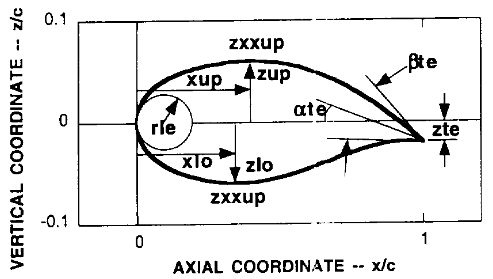
\includegraphics[width=0.5\linewidth]{figs/wing-ga.png}} 
    
    \small
    \begin{flushleft}
    \href{https://link.springer.com/chapter/10.1007/978-94-010-0017-8\_38\#citeas}{Holst T.L., Pulliam T.H. (2003) \textit{Transonic Wing Shape Optimization Using a Genetic Algorithm}. In: IUTAM Symposium Transsonicum IV. Fluid Mechanics and its Applications, vol 73. Springer.}
    \end{flushleft}
\end{frame}

\end{document}

    \end{columns}
\end{frame}

\section{Problem formulation}
\subsection{Types of problems}
\begin{frame}{Problem formulation}{Types of problems}
    %Search is a cornerstone in AI
    %\begin{itemize}
    %    \item Almost any problem in AI is formulated as a search problem
    %\end{itemize}

    Types of problems depending on ...
	\begin{itemize}
        \item Knowledge
            \begin{itemize}
                \item[-] Observable or Non-observable or Partially observable
            \end{itemize}
        \item Outcome
            \begin{itemize}
                \item[-] Deterministic or Stochastic
            \end{itemize}
        \item Actions
            \begin{itemize}
                \item[-] Discrete or Continous
            \end{itemize}
        \item Time-variance
            \begin{itemize}
                \item[-] Static or Dynamic
            \end{itemize}
	\end{itemize}
    We assume static, observable, discrete and deterministic problems
\end{frame}

\begin{frame}[fragile]{Problem formulation}{Types of problems (II)}
    \begin{exampleblock}{Determine problem type}
       \begin{columns}
 	       \column{.50\textwidth}
           \centering Chess\\
           \medskip
	        \includegraphics[width=0.75\linewidth]{figs/chess.png}\\

 	       \column{.50\textwidth}
           \centering League of Legends\\
           \medskip
	        \includegraphics[width=0.75\linewidth]{figs/lol.jpg}\\
        \end{columns}
        \medskip
        Observable or non-observable, deterministic or stochastic, discrete or continous, static or dynamic?
    \end{exampleblock}
\end{frame}

\subsection{Problem components}
\begin{frame}{Problem formulation}{Problem components (I)}
    We represent the environment as \alert{states}
        \begin{itemize}
            \item Contain the information about the world
        \end{itemize}
    Any problem formulation requires the following components
	\begin{itemize}
        \item \textbf{Initial state}: State where the search begins
        \item \textbf{Actions}: Behaviour that the agent may exhibit
        \item \textbf{Transition model}: Which states follow an action in a state (\alert{graph})
        \item \textbf{Goal test} (\textit{metas}): How to determine if a state is a goal
        \item \textbf{Path cost}: Cost of a path to a state
	\end{itemize}
\end{frame}

\begin{frame}{Problem formulation}{Problem components: Example (I)}
    \begin{center}
	    \includegraphics[width=0.7\linewidth]{figs/romania-distances.eps}\\
	    \tiny{\href{http://aima.cs.berkeley.edu/index.html}{(Source)}}
	\end{center}

    \begin{exampleblock}{Problem: Move from Arad to Bucharest}
        On holiday in Romania; currently in Arad, flight leaves tomorrow from Bucharest\\
        Determine: Initial state, goal, states, actions, transition model, goal test and path cost
    \end{exampleblock}
\end{frame}

\begin{frame}{Problem formulation}{Problem components: Example (II)}

       \begin{columns}
 	       \column{.60\textwidth}
    \begin{center}
	    \includegraphics[width=\linewidth]{figs/romania-distances.eps}\\
	    \tiny{\href{http://aima.cs.berkeley.edu/index.html}{(Source)}}
	\end{center}

 	       \column{.50\textwidth}
    \begin{exampleblock}{Solution}
        \begin{itemize}
            \item Initial state: Arad
            \item Goal: Bucharest
            \item States: Multiple cities
            \item Actions: Drive between cities
            \item Goal test: In Bucharest?
            \item Path cost: Distance
        \end{itemize}
    \end{exampleblock}

       \end{columns}
\end{frame}

\begin{frame}{Problem formulation}{Problem components: Search}
    \alert{Search} is the process of finding a solution
        \begin{itemize}
            \item A \alert{solution} is a sequence of actions leading from the initial state to a goal state
            \item \alert{Optimal solution} is a solution with the lowest cost
            \item Example of solution: Arad $\rightarrow$ Sibiu $\rightarrow$ Fagaras $\rightarrow$ Bucharest
                \begin{itemize}
                \item That solution is optimal?
                \end{itemize}
        \end{itemize}
\end{frame}


\subsection{Toy problems}
\begin{frame}[fragile]{Search problems}{Toy problems (I): Vacuum world}
       \begin{columns}
 	       \column{.40\textwidth}
	            \centering 
                \onslide<1> \includegraphics[width=\linewidth]{figs/vacuum2-environment.eps}\\
	            \tiny{\href{http://aima.cs.berkeley.edu/index.html}{(Source)}}

 	       \column{.60\textwidth}
                \begin{exampleblock}{Problem: Clean rooms}
                    \begin{itemize}
                    \item[-] State? $\rightarrow$ 
                    \item[-] Initial state? $\rightarrow$ 
                    \item[-] Goal? $\rightarrow$ 
                    \item[-] Actions? $\rightarrow$ 
                    \item[-] Transition model? $\rightarrow$ 
                    \item[-] Goal test? $\rightarrow$ 
                    \item[-] Path cost? $\rightarrow$
                    \end{itemize}
                \end{exampleblock}
      \end{columns}
\end{frame}

\begin{frame}[fragile]{Search problems}{Toy problems (I): Vacuum world}
       \begin{columns}
 	       \column{.40\textwidth}
	           \centering 
               \includegraphics[width=\linewidth]{figs/vacuum2-state-space.eps}\\
	           \tiny{\href{http://aima.cs.berkeley.edu/index.html}{(Source)}}

 	       \column{.60\textwidth}
                \begin{exampleblock}{Problem: Clean rooms}
                    \begin{itemize}
                    \item[-] State? $\rightarrow$ \textit{Dirt and location}
                    \item[-] Initial state? $\rightarrow$ \textit{All dirt, Left}
                    \item[-] Goal? $\rightarrow$ \textit{No dirt, any location}
                    \item[-] Actions? $\rightarrow$ \textit{Left, Right, Suck}
                    \item[-] Transition model? $\rightarrow$ \textit{See figure}
                    \item[-] Goal test? $\rightarrow$ \textit{No dirt, any location}
                    \item[-] Path cost? $\rightarrow$ \textit{1 per action}
                    \end{itemize}
                \end{exampleblock}
      \end{columns}
\end{frame}

\begin{frame}{Search problems}{Toy problems (II): 8-puzzle}
       \begin{columns}
 	       \column{.40\textwidth}
	            \centering \includegraphics[width=\linewidth]{figs/8puzzle.eps}\\
	            \tiny{\href{http://aima.cs.berkeley.edu/index.html}{(Source)}}
 	       \column{.60\textwidth}
                \begin{exampleblock}{Problem: Solve 8-puzzle}
                    \begin{itemize}
                    \item[-] State? $\rightarrow$ 
                    \item[-] Initial state? $\rightarrow$ 
                    \item[-] Goal? $\rightarrow$ 
                    \item[-] Actions? $\rightarrow$ 
                    \item[-] Transition model? $\rightarrow$ 
                    \item[-] Goal test? $\rightarrow$ 
                    \item[-] Path cost? $\rightarrow$
                    \end{itemize}
                \end{exampleblock}
      \end{columns}
\end{frame}

\begin{frame}{Search problems}{Toy problems (II): 8-puzzle}
       \begin{columns}
 	       \column{.40\textwidth}
	            \centering \includegraphics[width=\linewidth]{figs/8puzzle.eps}\\
	            \tiny{\href{http://aima.cs.berkeley.edu/index.html}{(Source)}}
 	       \column{.60\textwidth}
                \begin{exampleblock}{Problem: Solve 8-puzzle}
                    \begin{itemize}
                    \item[-] State? $\rightarrow$ \textit{Location of tiles}
                        \begin{itemize}
                            \item[] $9!/2 = 181,440$ states
                        \end{itemize}
                    \item[-] Initial state? $\rightarrow$ \textit{Any}
                    \item[-] Goal? $\rightarrow$ \textit{See figure}
                    \item[-] Actions? $\rightarrow$ \textit{Left, Right, Up, Down}
                    \item[-] Transition model? $\rightarrow$ Complex graph
                    \item[-] Goal test? $\rightarrow$ \textit{Goal state}
                    \item[-] Path cost? $\rightarrow$ \textit{1 per move}
                    \end{itemize}
                \end{exampleblock}

      \end{columns}
\end{frame}

\begin{frame}{Search problems}{Toy problems (III): 8-queens}
       \begin{columns}
 	       \column{.40\textwidth}
	            \centering \includegraphics[width=\linewidth]{figs/8queens.eps}\\
	            \tiny{\href{http://aima.cs.berkeley.edu/index.html}{(Source)}}
 	       \column{.60\textwidth}
                \begin{exampleblock}{Problem: Place 8 queens no queen attacks any other}
                State?\\
                Initial state? \\
                Goal? \\
                Actions? \\ 
                Transition model? \\
                Goal test? \\
                Path cost?\\
                \end{exampleblock}
      \end{columns}
\end{frame}

\begin{frame}{Search problems}{Toy problems (III): 8-queens}
       \begin{columns}
 	       \column{.40\textwidth}
	            \centering \includegraphics[width=\linewidth]{figs/8queens.eps}\\
	            \tiny{\href{http://aima.cs.berkeley.edu/index.html}{(Source)}}
 	       \column{.60\textwidth}
                \begin{exampleblock}{Problem: Place 8 queens no queen attacks any other}
                    \begin{itemize}
                    \item[-] State? $\rightarrow$ \textit{Any arrangement of 0 to 8 queens}
                    \item[-] Initial state? $\rightarrow$ \textit{Empty board}
                    \item[-] Goal? $\rightarrow$ \textit{See figure}
                    \item[-] Actions? $\rightarrow$ \textit{Add queen to empty square}
                    \item[-] Transition model? $\rightarrow$ Complex graph
                    \item[-] Goal test? $\rightarrow$ \textit{8 queens on board, none attacked}
                    \item[-] Path cost? $\rightarrow$ \textit{1 per move}
                    \end{itemize}
                \end{exampleblock}
      \end{columns}
\end{frame}

\subsection{Travel Salesman Problem}
\begin{frame}{Search problems}{Travelling Salesman Problem (TSP)}
       \begin{columns}
 	       \column{.50\textwidth}
                \begin{block}{TSP formulation}
                    A travelling salesman must visit a set of cities only one time each. Find the shortest route.
                \end{block}

                TSP is a very big problem in AI!
                \begin{itemize}
                    \item First formulated in 1930 and still a hot research topic!
                    \item NP-hard problem
                    \item Many real world applications
                \end{itemize}

 	       \column{.50\textwidth}
                \centering 
                \begin{tikzpicture}[scale=0.6]
                    \node[shape=circle, draw] (A) at (0,0) {A};
                    \node[shape=circle, draw] (B) at (0,3) {B};
                    \node[shape=circle, draw] (C) at (2.5,4) {C};
                    \node[shape=circle, draw] (D) at (2.5,1) {D};
                    \node[shape=circle, draw] (E) at (2.5,-2) {E};
                    \node[shape=circle, draw] (F) at (5,3) {F} ;

                    \path [-] (A) edge node[left] {$5$} (B);
                    \path [-](B) edge node[left] {$3$} (C);
                    \path [-](A) edge node[left] {$4$} (D);
                    \path [-](D) edge node[left] {$3$} (C);
                    \path [-](A) edge node[right] {$3$} (E);
                    \path [-](D) edge node[left] {$3$} (E);
                    \path [-](D) edge node {$3$} (F);
                    \path [-](C) edge node {$5$} (F);
                    \path [-](E) edge node[right] {$8$} (F); 
                \end{tikzpicture}

                \tiny{\href{https://tex.stackexchange.com/questions/270543/draw-a-graph-in-latex-with-tikz}{(Source)}}
      \end{columns}
\end{frame}

\section{Search strategy}

\begin{frame}{Search strategy (I)}
    In general ...
	    \begin{itemize}
    	    \item Each problem has a search graph, or \textbf{state space}
        	\item Searching means finding a path from the initial state to a goal state
    	\end{itemize}

    Basic idea
        \begin{itemize}
            \item Explore search space
            \item Generate a \textbf{search tree} (i.e., \textbf{expanding nodes})
        \end{itemize}

    A search strategy is defined by picking the order of node exansion
        \begin{itemize}
            \item Uninformed search: Only uses the problem definition
            \item Informed search: Uses problem-specific knowledge
        \end{itemize}
\end{frame}

\begin{frame}{Search strategy (II)}
    Search strategies are evaluated along the following dimensions
	    \begin{itemize}
    	    \item Completeness
        	\item Time complexity
            \item Space complexity
            \item Optimality
    	\end{itemize}

    Time and space are measured in terms of 
        \begin{itemize}
            \item b: Maximum branching factor
            \item d: Depth of the least-cost solution
            \item m: Maximum depth of the state space
        \end{itemize}
\end{frame}

\section{Uninformed search}
%\subsection{Introduction}

\begin{frame}{Uninformed search}
    Uninformed search algorithms
    \begin{itemize}
        \item Breadth-first search (\textit{búsqueda en anchura})
        \item Uniform-cost search (\textit{búsqueda de coste uniforme})
        \item Depth-first search (\textit{búsqueda en profundidad})
        \item Depth-limited search (\textit{búsqueda en profundidad limitada})
        \item Iterative deepening search (\textit{búsqueda de profundización iterativa})
    \end{itemize}
\end{frame}

\subsection{Breadth-first search}

\begin{frame}{Uninformed search}{Breadth-first search (I)}
      Expand shallowest unexpanded node
      \begin{itemize}
        \item Implemented with a FIFO queue (First-In First-Out)
      \end{itemize}

      \bigskip 

      \begin{center}
          \includegraphics[width=\linewidth]{figs/bfs-progress.eps}\\
          \tiny{\href{http://aima.cs.berkeley.edu/index.html}{(Source)}}
      \end{center}
\end{frame}

\begin{frame}{Uninformed search}{Breadth-first search (II)}
      \begin{center}
          \setlength{\fboxrule}{0pt}
          \fbox{\includegraphics[natwidth=1124bp,natheight=462bp, width=0.7\linewidth]{figs/20-Figure3.13-1.png}} \\
          %\includegraphics[natwidth=1124, natwidth=462]{figs/20-Figure3.13-1.png}\\
          \tiny{\href{http://aima.cs.berkeley.edu/index.html}{(Source)}}
      \end{center}

      \bigskip

      Properties of breadth-first search
      \begin{itemize}
        \item Completeness: Yes
        \item Time complexity: $O(b^{d+1})$
        \item Space complexity: $O(b^{d+1})$
        \item Optimality: Yes (if cost = 1 per step)
      \end{itemize}
      Space is the biggest problem (more than time)
\end{frame}

\subsection{Uniform-cost search}

\begin{frame}{Uninformed search}{Uniform-cost search (I)}
    Special case of breadth-first search
    \begin{itemize}
        \item Expand least-cost unexpanded node
        \item The queue is sorted by cost
    \end{itemize}

    \begin{columns}
 	       \column{.50\textwidth}
                \setlength{\fboxrule}{0pt}
                \fbox{\includegraphics[width=\linewidth]{figs/Grafo1.png}} 
 	       \column{.50\textwidth}
                \setlength{\fboxrule}{0pt}
                \fbox{\includegraphics[width=0.7\linewidth]{figs/Grafo2.png}} 
    \end{columns}
\end{frame}

\begin{frame}[fragile]{Uninformed search}{Uniform-cost search (II)}
    \begin{exampleblock}{Uniform-cost example}
    \small{
    Initialization: $\{[S, 0]\}$\\
    Iter. 1: $\{[S \rightarrow A, 1], [S \rightarrow G, 12]\}$\\
    Iter. 2: $\{[S \rightarrow A \rightarrow C, 2], [S \rightarrow A \rightarrow B, 4], [S \rightarrow G, 12]\}$\\
    Iter. 3: $\{[S \rightarrow A \rightarrow C \rightarrow D, 3], [S \rightarrow A \rightarrow C \rightarrow G, 4], [S \rightarrow A \rightarrow B \rightarrow D, 7], [S \rightarrow G, 12]\}$\\
    Iter. 4: $\{[S \rightarrow A \rightarrow C \rightarrow D \rightarrow G, 6], [S \rightarrow A \rightarrow C \rightarrow G, 4], [S \rightarrow A \rightarrow B \rightarrow D, 7], [S \rightarrow G, 12]\}$\\
    Iter. 5: $\{[S \rightarrow A \rightarrow C \rightarrow G, 4], [S \rightarrow A \rightarrow C \rightarrow D \rightarrow G, 10], [S \rightarrow G, 12]\}$\\
    Solution: $S \rightarrow A \rightarrow C \rightarrow G$\\
    }
    \end{exampleblock}
\end{frame}

\begin{frame}[fragile]{Uninformed search}{Uniform-cost search (III)}
      Properties
      \begin{itemize}
        \item Completeness: Yes, if step cost $\ge\epsilon$
        \item Time complexity: $O(b^{\lceil C^{*}/\epsilon \rceil})$, where $C^{*}$ is the cost of the optimal solution
        \item Space complexity: $O(b^{\lceil C^{*}/\epsilon \rceil})$
        \item Optimality: Yes
      \end{itemize}
      Space is the biggest problem (more than time)
\end{frame}

\subsection{Depth-first search}

\begin{frame}{Uninformed search}{Depth-first search (I)}
    Expand deepest unexpanded node
    \begin{itemize}
        \item Implemented with a LIFO stack
    \end{itemize}
\end{frame}

\begin{frame}[plain]
      \begin{center}
          \includegraphics[width=\linewidth]{figs/dfs-progress-noblack.eps}\\
          \tiny{\href{http://aima.cs.berkeley.edu/index.html}{(Source)}}
      \end{center}
\end{frame}

\begin{frame}{Uninformed search}{Depth-first search (III)}
      Properties of depth-first search
      \begin{itemize}
        \item Completeness: No, fail in infinite-depth spaces or spaces with loops
        \item Time complexity: $O(b^{m})$, (terrible if $m>>d$)
        \item Space complexity: $O(bm)$
        \item Optimality: No
      \end{itemize}
\end{frame}

\subsection{Depth-limited search}

\begin{frame}{Uninformed search}{Depth-limited search}
      Depth-first search with depth limit L
      \begin{itemize}
        \item Nodes at depth L are not expanded
      \end{itemize}
\end{frame}

\subsection{Iterative deepening depth-first search}

\begin{frame}{Uninformed search}{Iterative deepening depth-first search (I)}
    Depth-limited search where gradually increases L
\end{frame}

\begin{frame}[plain,shrink]
      \begin{center}
          \includegraphics[width=\linewidth]{figs/ids-progress.eps}\\
          \tiny{\href{http://aima.cs.berkeley.edu/index.html}{(Source)}}
      \end{center}
\end{frame}

\begin{frame}{Uninformed search}{Iterative deepening depth-first search (III)}
      Properties
      \begin{itemize}
        \item Completeness: Yes
        \item Time complexity: $O(b^{d})$
        \item Space complexity: $O(bd)$
        \item Optimality: Yes if step cost = 1
      \end{itemize}
\end{frame}


\subsection{Comparison of uninformed search algorithms}

\begin{frame}{Uninformed search}{Comparison of uninformed search algorithms}

\begin{tabular}{cccccc}
\hline
Criterion & Breadth- & Uniform- & Depth- & Depth- & Iterative \\
          & First &  Cost & First & Limited & Deepening \\
\hline
Complete  & Yes$^*$ & Yes$^*$ & No & Yes, if $l \ge d$ & Yes \\
Time      & $b^{d+1}$ & $b^{\lceil C^*/\epsilon \rceil}$ & $b^m$ & $b^l$ & $b^d$ \\
Space     & $b^{d+1}$ & $b^{\lceil C^*/\epsilon \rceil}$ & $bm$ & $bl$ & $bd$ \\
Optimal   & Yes$^*$ & Yes & No & No & Yes$^*$ \\
\hline
\end{tabular}

\end{frame}


\section{Informed search}
\subsection{Introduction}

\begin{frame}{Informed search}{Introduction (I)}
    Use problem-specific knowledge beyond problem definition
      \begin{itemize}
        \item Best-first search (\textit{búsqueda primero el mejor})
            \begin{itemize}
                \item Greedy best-first search (\textit{Búsqueda voraz})
                \item A* search
            \end{itemize}
        \item Local search algorithms
            \begin{itemize}
            \item Hill-climbing search (\textit{búsqueda en escalada})
            \item Simulated annealing search (\textit{búsqueda de temple simulado})
            \item Local beam search (\textit{búsqueda de haz local})
            \item Genetic Algorithms 
        \end{itemize}
      \end{itemize}
\end{frame}

\begin{frame}{Informed search}{Introduction (II)}
    Best-first search
      \begin{itemize}
        \item Use an evaluation function $f(n)$ for each node
        \item Estimate of ``desirability''
        \item Expand most desirable unexpanded nodes
      \end{itemize}

    Most algorithms use a \alert{heuristic function} or just \alert{heuristic} ($h(n)$)
      \begin{itemize}
        \item Estimated cost from a state to the goal
      \end{itemize}

    Best-first algorithms
      \begin{itemize}
        \item Greedy best-first search
        \item A*
      \end{itemize}
\end{frame}

\subsection{Greedy best-first search}

\begin{frame}{Informed search}{Greedy best-first search (I)}
    \begin{columns}
 	    \column{.50\textwidth}
            It only considers the heuristic
            \begin{itemize}
                \item Greedy search expands the node that \textit{appears} to be closest to the goal
            \end{itemize}

 	    \column{.50\textwidth}
            \begin{block}{Greedy search}
                $f(n) = h (n)$
            \end{block}
    \end{columns}
    
    \bigskip

    Example: Find a path between Arad and Bucharest
    \begin{itemize}
        \item Heuristic: Straight-line distance
    \end{itemize}

    \centering \includegraphics[width=0.6\linewidth]{figs/romania-distances.eps}\\
    \tiny{\href{http://aima.cs.berkeley.edu/index.html}{(Source)}}
\end{frame}

\begin{frame}[plain,shrink]
      \begin{center}
          \includegraphics[width=\linewidth]{figs/greedy-progress.eps}\\
          \tiny{\href{http://aima.cs.berkeley.edu/index.html}{(Source)}}
      \end{center}
\end{frame}

\subsection{A*}

\begin{frame}{Informed search}{A* (I)}
    \begin{columns}
 	    \column{.50\textwidth}
            It considers the heuristic and the cost
            \begin{itemize}
                \item $h(n)$: Estimated cost to goal from node n
                \item $g(n)$: Cost to node n
            \end{itemize}

 	    \column{.50\textwidth}
            \begin{block}{A*}
                $f(n) = g(n) + h (n)$
            \end{block}
    \end{columns}

    \bigskip

    Theorem: A* is optimal if $h(n)$ is \alert{admisible}
        \begin{itemize}
        \item A* is admisible if it never overestimates the cost
        \item Example: Straight-line distance never overestimates road distance
        \end{itemize}
    \bigskip
\end{frame}

\begin{frame}[plain,shrink]
      \begin{center}
          \quad \includegraphics[width=\linewidth]{figs/astar-progress.eps}\\
          \tiny{\href{http://aima.cs.berkeley.edu/index.html}{(Source)}}
      \end{center}
\end{frame}

\begin{frame}{Informed search}{A* (III)}
      Properties
      \begin{itemize}
        \item Completeness: Yes
        \item Time complexity: Exponential
        \item Space complexity: Keeps all nodes in memory
        \item Optimality: Yes
      \end{itemize}
\end{frame}

\section{Case studies}
%\subsection{Case study I: Robotic assembly}

%\begin{frame}{Case studies}{Case study I: Robotic assembly}
%       \begin{columns}
%	       \column{.60\textwidth}
%            \centering \includegraphics[width=\linewidth]{figs/stanford-arm.eps}\\
%            \tiny{\href{http://aima.cs.berkeley.edu/index.html}{(Source)}}
%	       \column{.40\textwidth}
%               \begin{exampleblock}{Problem: Robotic assembly}
%                   \begin{itemize}
%                   \item[-] State? $\rightarrow$ \textit{Real-valued coordinates of robot joint angles}
%                   \item[-] Actions? $\rightarrow$ \textit{Continuous motions of joints}
%                   \item[-] Goal test? $\rightarrow$ \textit{Complete assembly}
%                   \item[-] Path cost? $\rightarrow$ \textit{Time to complete}
%                   \end{itemize}
%               \end{exampleblock}

%     \end{columns}
%end{frame}

\subsection{Case study I: Robot arm with two DOF}
\begin{frame}{Case studies}{Case study I: Robot arm with two DOF (I)}
       \begin{columns}
 	       \column{.50\textwidth}
	            \centering \includegraphics[width=\linewidth]{figs/armPlain.eps}\\
	            \tiny{\href{http://aima.cs.berkeley.edu/index.html}{(Source)}}
 	       \column{.50\textwidth}
                \begin{exampleblock}{Problem: Move arm}
                    \begin{itemize}
                    \item[-] State? $\rightarrow$ 
                    \item[-] Actions? $\rightarrow$ 
                    \item[-] Goal test? $\rightarrow$ 
                    \item[-] Path cost? $\rightarrow$
                    \end{itemize}
                \end{exampleblock}
      \end{columns}
\end{frame}

\begin{frame}{Case studies}{Case study I: Robot arm with two DOF (I)}
       \begin{columns}
 	       \column{.50\textwidth}
	            \centering \includegraphics[width=\linewidth]{figs/armPlain.eps}\\
	            \tiny{\href{http://aima.cs.berkeley.edu/index.html}{(Source)}}
 	       \column{.50\textwidth}
                \begin{exampleblock}{Problem: Move arm}
                    \begin{itemize}
                    \item[-] State? $\rightarrow$ \textit{Real-valued coordinates of robot joint angles}
                    \item[-] Actions? $\rightarrow$ \textit{Continuous motions of joints}
                    \item[-] Goal test? $\rightarrow$ \textit{Complete assembly}
                    \item[-] Path cost? $\rightarrow$ \textit{Time to complete}
                    \end{itemize}
                \end{exampleblock}
      \end{columns}
\end{frame}



\begin{frame}{Case studies}{Case study I: Robot arm with two DOF (II)}
       \begin{columns}
 	       \column{.50\textwidth}
            \centering \includegraphics[width=\linewidth]{figs/armPlain.eps}\\
	       \column{.50\textwidth}
            \centering \includegraphics[width=\linewidth]{figs/armPlainConfSpace.eps}\\
     \end{columns}
  \centering \tiny{\href{http://aima.cs.berkeley.edu/index.html}{(Source)}}
\end{frame}

\begin{frame}{Case studies}{Case study I: Robot arm with two DOF (III)}
       \begin{columns}
 	       \column{.50\textwidth}
	            \centering \includegraphics[width=\linewidth]{figs/armExampleWorkSpace.eps}\\
 	       \column{.50\textwidth}
	            \centering \includegraphics[width=\linewidth]{figs/armExampleConfSpace.eps}\\
      \end{columns}
	  \centering \tiny{\href{http://aima.cs.berkeley.edu/index.html}{(Source)}}
\end{frame}

\begin{frame}{Case studies}{Case study I: Robot arm with two DOF (IV)}
       \begin{columns}
 	       \column{.50\textwidth}
	            \centering \includegraphics[width=\linewidth]{figs/armDPwithoutPotentialWorkspaceCoarse.eps}\\
 	       \column{.50\textwidth}
	            \centering \includegraphics[width=\linewidth]{figs/armDPwithoutPotentialCoarse.eps}\\
      \end{columns}
	  \centering \tiny{\href{http://aima.cs.berkeley.edu/index.html}{(Source)}}
\end{frame}

\subsection{Case study II: 9\textsuperscript{th} GTOC}
\begin{frame}{Study case}{Case study II: 9\textsuperscript{th} Global Trajectory Optimization Competition (I)}
    GTOC: Global Trajectory Optimization Competition
    \begin{itemize}
        \item Proposed by ESA Advanced Concepts Team
        \item Difficult trajectory optimization problems
    \end{itemize}

    GTOC 9: The Kesser Run
    \begin{itemize}
        \item 123 orbiting debris
        \item Remove debris
        \item Design multiple missions
    \end{itemize}
    \href{https://www.youtube.com/watch?v=zvxZx-QnqQ0}{(Video)}
    \href{https://www.youtube.com/watch?v=5CQNG6OIbZM}{(Solution)}
\end{frame}

\subsection{Case study III: Mars orbital insertion}
\begin{frame}{Study case}{Case study III: Mars orbital insertion}
    \setlength{\fboxrule}{0pt}
    \fbox{\includegraphics[width=0.7\linewidth]{figs/orbits.jpg}} 
\end{frame}

\subsection{Case study IV: Transonic wing shape optimization}
\begin{frame}{Study case}{Case study IV: Transonic wing shape optimization}
    Problem: Design a wing shape for transonic flight
        \begin{itemize}
        \item Maximize lift
        \end{itemize}

    \setlength{\fboxrule}{0pt}
    \centering \fbox{\includegraphics[width=0.5\linewidth]{figs/wing-ga.png}} 
    
    \small
    \begin{flushleft}
    \href{https://link.springer.com/chapter/10.1007/978-94-010-0017-8\_38\#citeas}{Holst T.L., Pulliam T.H. (2003) \textit{Transonic Wing Shape Optimization Using a Genetic Algorithm}. In: IUTAM Symposium Transsonicum IV. Fluid Mechanics and its Applications, vol 73. Springer.}
    \end{flushleft}
\end{frame}

\end{document}

    \end{columns}
\end{frame}

\section{Problem formulation}
\subsection{Types of problems}
\begin{frame}{Problem formulation}{Types of problems}
    %Search is a cornerstone in AI
    %\begin{itemize}
    %    \item Almost any problem in AI is formulated as a search problem
    %\end{itemize}

    Types of problems depending on ...
	\begin{itemize}
        \item Knowledge
            \begin{itemize}
                \item[-] Observable or Non-observable or Partially observable
            \end{itemize}
        \item Outcome
            \begin{itemize}
                \item[-] Deterministic or Stochastic
            \end{itemize}
        \item Actions
            \begin{itemize}
                \item[-] Discrete or Continous
            \end{itemize}
        \item Time-variance
            \begin{itemize}
                \item[-] Static or Dynamic
            \end{itemize}
	\end{itemize}
    We assume static, observable, discrete and deterministic problems
\end{frame}

\begin{frame}[fragile]{Problem formulation}{Types of problems (II)}
    \begin{exampleblock}{Determine problem type}
       \begin{columns}
 	       \column{.50\textwidth}
           \centering Chess\\
           \medskip
	        \includegraphics[width=0.75\linewidth]{figs/chess.png}\\

 	       \column{.50\textwidth}
           \centering League of Legends\\
           \medskip
	        \includegraphics[width=0.75\linewidth]{figs/lol.jpg}\\
        \end{columns}
        \medskip
        Observable or non-observable, deterministic or stochastic, discrete or continous, static or dynamic?
    \end{exampleblock}
\end{frame}

\subsection{Problem components}
\begin{frame}{Problem formulation}{Problem components (I)}
    We represent the environment as \alert{states}
        \begin{itemize}
            \item Contain the information about the world
        \end{itemize}
    Any problem formulation requires the following components
	\begin{itemize}
        \item \textbf{Initial state}: State where the search begins
        \item \textbf{Actions}: Behaviour that the agent may exhibit
        \item \textbf{Transition model}: Which states follow an action in a state (\alert{graph})
        \item \textbf{Goal test} (\textit{metas}): How to determine if a state is a goal
        \item \textbf{Path cost}: Cost of a path to a state
	\end{itemize}
\end{frame}

\begin{frame}{Problem formulation}{Problem components: Example (I)}
    \begin{center}
	    \includegraphics[width=0.7\linewidth]{figs/romania-distances.eps}\\
	    \tiny{\href{http://aima.cs.berkeley.edu/index.html}{(Source)}}
	\end{center}

    \begin{exampleblock}{Problem: Move from Arad to Bucharest}
        On holiday in Romania; currently in Arad, flight leaves tomorrow from Bucharest\\
        Determine: Initial state, goal, states, actions, transition model, goal test and path cost
    \end{exampleblock}
\end{frame}

\begin{frame}{Problem formulation}{Problem components: Example (II)}

       \begin{columns}
 	       \column{.60\textwidth}
    \begin{center}
	    \includegraphics[width=\linewidth]{figs/romania-distances.eps}\\
	    \tiny{\href{http://aima.cs.berkeley.edu/index.html}{(Source)}}
	\end{center}

 	       \column{.50\textwidth}
    \begin{exampleblock}{Solution}
        \begin{itemize}
            \item Initial state: Arad
            \item Goal: Bucharest
            \item States: Multiple cities
            \item Actions: Drive between cities
            \item Goal test: In Bucharest?
            \item Path cost: Distance
        \end{itemize}
    \end{exampleblock}

       \end{columns}
\end{frame}

\begin{frame}{Problem formulation}{Problem components: Search}
    \alert{Search} is the process of finding a solution
        \begin{itemize}
            \item A \alert{solution} is a sequence of actions leading from the initial state to a goal state
            \item \alert{Optimal solution} is a solution with the lowest cost
            \item Example of solution: Arad $\rightarrow$ Sibiu $\rightarrow$ Fagaras $\rightarrow$ Bucharest
                \begin{itemize}
                \item That solution is optimal?
                \end{itemize}
        \end{itemize}
\end{frame}


\subsection{Toy problems}
\begin{frame}[fragile]{Search problems}{Toy problems (I): Vacuum world}
       \begin{columns}
 	       \column{.40\textwidth}
	            \centering 
                \onslide<1> \includegraphics[width=\linewidth]{figs/vacuum2-environment.eps}\\
	            \tiny{\href{http://aima.cs.berkeley.edu/index.html}{(Source)}}

 	       \column{.60\textwidth}
                \begin{exampleblock}{Problem: Clean rooms}
                    \begin{itemize}
                    \item[-] State? $\rightarrow$ 
                    \item[-] Initial state? $\rightarrow$ 
                    \item[-] Goal? $\rightarrow$ 
                    \item[-] Actions? $\rightarrow$ 
                    \item[-] Transition model? $\rightarrow$ 
                    \item[-] Goal test? $\rightarrow$ 
                    \item[-] Path cost? $\rightarrow$
                    \end{itemize}
                \end{exampleblock}
      \end{columns}
\end{frame}

\begin{frame}[fragile]{Search problems}{Toy problems (I): Vacuum world}
       \begin{columns}
 	       \column{.40\textwidth}
	           \centering 
               \includegraphics[width=\linewidth]{figs/vacuum2-state-space.eps}\\
	           \tiny{\href{http://aima.cs.berkeley.edu/index.html}{(Source)}}

 	       \column{.60\textwidth}
                \begin{exampleblock}{Problem: Clean rooms}
                    \begin{itemize}
                    \item[-] State? $\rightarrow$ \textit{Dirt and location}
                    \item[-] Initial state? $\rightarrow$ \textit{All dirt, Left}
                    \item[-] Goal? $\rightarrow$ \textit{No dirt, any location}
                    \item[-] Actions? $\rightarrow$ \textit{Left, Right, Suck}
                    \item[-] Transition model? $\rightarrow$ \textit{See figure}
                    \item[-] Goal test? $\rightarrow$ \textit{No dirt, any location}
                    \item[-] Path cost? $\rightarrow$ \textit{1 per action}
                    \end{itemize}
                \end{exampleblock}
      \end{columns}
\end{frame}

\begin{frame}{Search problems}{Toy problems (II): 8-puzzle}
       \begin{columns}
 	       \column{.40\textwidth}
	            \centering \includegraphics[width=\linewidth]{figs/8puzzle.eps}\\
	            \tiny{\href{http://aima.cs.berkeley.edu/index.html}{(Source)}}
 	       \column{.60\textwidth}
                \begin{exampleblock}{Problem: Solve 8-puzzle}
                    \begin{itemize}
                    \item[-] State? $\rightarrow$ 
                    \item[-] Initial state? $\rightarrow$ 
                    \item[-] Goal? $\rightarrow$ 
                    \item[-] Actions? $\rightarrow$ 
                    \item[-] Transition model? $\rightarrow$ 
                    \item[-] Goal test? $\rightarrow$ 
                    \item[-] Path cost? $\rightarrow$
                    \end{itemize}
                \end{exampleblock}
      \end{columns}
\end{frame}

\begin{frame}{Search problems}{Toy problems (II): 8-puzzle}
       \begin{columns}
 	       \column{.40\textwidth}
	            \centering \includegraphics[width=\linewidth]{figs/8puzzle.eps}\\
	            \tiny{\href{http://aima.cs.berkeley.edu/index.html}{(Source)}}
 	       \column{.60\textwidth}
                \begin{exampleblock}{Problem: Solve 8-puzzle}
                    \begin{itemize}
                    \item[-] State? $\rightarrow$ \textit{Location of tiles}
                        \begin{itemize}
                            \item[] $9!/2 = 181,440$ states
                        \end{itemize}
                    \item[-] Initial state? $\rightarrow$ \textit{Any}
                    \item[-] Goal? $\rightarrow$ \textit{See figure}
                    \item[-] Actions? $\rightarrow$ \textit{Left, Right, Up, Down}
                    \item[-] Transition model? $\rightarrow$ Complex graph
                    \item[-] Goal test? $\rightarrow$ \textit{Goal state}
                    \item[-] Path cost? $\rightarrow$ \textit{1 per move}
                    \end{itemize}
                \end{exampleblock}

      \end{columns}
\end{frame}

\begin{frame}{Search problems}{Toy problems (III): 8-queens}
       \begin{columns}
 	       \column{.40\textwidth}
	            \centering \includegraphics[width=\linewidth]{figs/8queens.eps}\\
	            \tiny{\href{http://aima.cs.berkeley.edu/index.html}{(Source)}}
 	       \column{.60\textwidth}
                \begin{exampleblock}{Problem: Place 8 queens no queen attacks any other}
                State?\\
                Initial state? \\
                Goal? \\
                Actions? \\ 
                Transition model? \\
                Goal test? \\
                Path cost?\\
                \end{exampleblock}
      \end{columns}
\end{frame}

\begin{frame}{Search problems}{Toy problems (III): 8-queens}
       \begin{columns}
 	       \column{.40\textwidth}
	            \centering \includegraphics[width=\linewidth]{figs/8queens.eps}\\
	            \tiny{\href{http://aima.cs.berkeley.edu/index.html}{(Source)}}
 	       \column{.60\textwidth}
                \begin{exampleblock}{Problem: Place 8 queens no queen attacks any other}
                    \begin{itemize}
                    \item[-] State? $\rightarrow$ \textit{Any arrangement of 0 to 8 queens}
                    \item[-] Initial state? $\rightarrow$ \textit{Empty board}
                    \item[-] Goal? $\rightarrow$ \textit{See figure}
                    \item[-] Actions? $\rightarrow$ \textit{Add queen to empty square}
                    \item[-] Transition model? $\rightarrow$ Complex graph
                    \item[-] Goal test? $\rightarrow$ \textit{8 queens on board, none attacked}
                    \item[-] Path cost? $\rightarrow$ \textit{1 per move}
                    \end{itemize}
                \end{exampleblock}
      \end{columns}
\end{frame}

\subsection{Travel Salesman Problem}
\begin{frame}{Search problems}{Travelling Salesman Problem (TSP)}
       \begin{columns}
 	       \column{.50\textwidth}
                \begin{block}{TSP formulation}
                    A travelling salesman must visit a set of cities only one time each. Find the shortest route.
                \end{block}

                TSP is a very big problem in AI!
                \begin{itemize}
                    \item First formulated in 1930 and still a hot research topic!
                    \item NP-hard problem
                    \item Many real world applications
                \end{itemize}

 	       \column{.50\textwidth}
                \centering 
                \begin{tikzpicture}[scale=0.6]
                    \node[shape=circle, draw] (A) at (0,0) {A};
                    \node[shape=circle, draw] (B) at (0,3) {B};
                    \node[shape=circle, draw] (C) at (2.5,4) {C};
                    \node[shape=circle, draw] (D) at (2.5,1) {D};
                    \node[shape=circle, draw] (E) at (2.5,-2) {E};
                    \node[shape=circle, draw] (F) at (5,3) {F} ;

                    \path [-] (A) edge node[left] {$5$} (B);
                    \path [-](B) edge node[left] {$3$} (C);
                    \path [-](A) edge node[left] {$4$} (D);
                    \path [-](D) edge node[left] {$3$} (C);
                    \path [-](A) edge node[right] {$3$} (E);
                    \path [-](D) edge node[left] {$3$} (E);
                    \path [-](D) edge node {$3$} (F);
                    \path [-](C) edge node {$5$} (F);
                    \path [-](E) edge node[right] {$8$} (F); 
                \end{tikzpicture}

                \tiny{\href{https://tex.stackexchange.com/questions/270543/draw-a-graph-in-latex-with-tikz}{(Source)}}
      \end{columns}
\end{frame}

\section{Search strategy}

\begin{frame}{Search strategy (I)}
    In general ...
	    \begin{itemize}
    	    \item Each problem has a search graph, or \textbf{state space}
        	\item Searching means finding a path from the initial state to a goal state
    	\end{itemize}

    Basic idea
        \begin{itemize}
            \item Explore search space
            \item Generate a \textbf{search tree} (i.e., \textbf{expanding nodes})
        \end{itemize}

    A search strategy is defined by picking the order of node exansion
        \begin{itemize}
            \item Uninformed search: Only uses the problem definition
            \item Informed search: Uses problem-specific knowledge
        \end{itemize}
\end{frame}

\begin{frame}{Search strategy (II)}
    Search strategies are evaluated along the following dimensions
	    \begin{itemize}
    	    \item Completeness
        	\item Time complexity
            \item Space complexity
            \item Optimality
    	\end{itemize}

    Time and space are measured in terms of 
        \begin{itemize}
            \item b: Maximum branching factor
            \item d: Depth of the least-cost solution
            \item m: Maximum depth of the state space
        \end{itemize}
\end{frame}

\section{Uninformed search}
%\subsection{Introduction}

\begin{frame}{Uninformed search}
    Uninformed search algorithms
    \begin{itemize}
        \item Breadth-first search (\textit{búsqueda en anchura})
        \item Uniform-cost search (\textit{búsqueda de coste uniforme})
        \item Depth-first search (\textit{búsqueda en profundidad})
        \item Depth-limited search (\textit{búsqueda en profundidad limitada})
        \item Iterative deepening search (\textit{búsqueda de profundización iterativa})
    \end{itemize}
\end{frame}

\subsection{Breadth-first search}

\begin{frame}{Uninformed search}{Breadth-first search (I)}
      Expand shallowest unexpanded node
      \begin{itemize}
        \item Implemented with a FIFO queue (First-In First-Out)
      \end{itemize}

      \bigskip 

      \begin{center}
          \includegraphics[width=\linewidth]{figs/bfs-progress.eps}\\
          \tiny{\href{http://aima.cs.berkeley.edu/index.html}{(Source)}}
      \end{center}
\end{frame}

\begin{frame}{Uninformed search}{Breadth-first search (II)}
      \begin{center}
          \setlength{\fboxrule}{0pt}
          \fbox{\includegraphics[natwidth=1124bp,natheight=462bp, width=0.7\linewidth]{figs/20-Figure3.13-1.png}} \\
          %\includegraphics[natwidth=1124, natwidth=462]{figs/20-Figure3.13-1.png}\\
          \tiny{\href{http://aima.cs.berkeley.edu/index.html}{(Source)}}
      \end{center}

      \bigskip

      Properties of breadth-first search
      \begin{itemize}
        \item Completeness: Yes
        \item Time complexity: $O(b^{d+1})$
        \item Space complexity: $O(b^{d+1})$
        \item Optimality: Yes (if cost = 1 per step)
      \end{itemize}
      Space is the biggest problem (more than time)
\end{frame}

\subsection{Uniform-cost search}

\begin{frame}{Uninformed search}{Uniform-cost search (I)}
    Special case of breadth-first search
    \begin{itemize}
        \item Expand least-cost unexpanded node
        \item The queue is sorted by cost
    \end{itemize}

    \begin{columns}
 	       \column{.50\textwidth}
                \setlength{\fboxrule}{0pt}
                \fbox{\includegraphics[width=\linewidth]{figs/Grafo1.png}} 
 	       \column{.50\textwidth}
                \setlength{\fboxrule}{0pt}
                \fbox{\includegraphics[width=0.7\linewidth]{figs/Grafo2.png}} 
    \end{columns}
\end{frame}

\begin{frame}[fragile]{Uninformed search}{Uniform-cost search (II)}
    \begin{exampleblock}{Uniform-cost example}
    \small{
    Initialization: $\{[S, 0]\}$\\
    Iter. 1: $\{[S \rightarrow A, 1], [S \rightarrow G, 12]\}$\\
    Iter. 2: $\{[S \rightarrow A \rightarrow C, 2], [S \rightarrow A \rightarrow B, 4], [S \rightarrow G, 12]\}$\\
    Iter. 3: $\{[S \rightarrow A \rightarrow C \rightarrow D, 3], [S \rightarrow A \rightarrow C \rightarrow G, 4], [S \rightarrow A \rightarrow B \rightarrow D, 7], [S \rightarrow G, 12]\}$\\
    Iter. 4: $\{[S \rightarrow A \rightarrow C \rightarrow D \rightarrow G, 6], [S \rightarrow A \rightarrow C \rightarrow G, 4], [S \rightarrow A \rightarrow B \rightarrow D, 7], [S \rightarrow G, 12]\}$\\
    Iter. 5: $\{[S \rightarrow A \rightarrow C \rightarrow G, 4], [S \rightarrow A \rightarrow C \rightarrow D \rightarrow G, 10], [S \rightarrow G, 12]\}$\\
    Solution: $S \rightarrow A \rightarrow C \rightarrow G$\\
    }
    \end{exampleblock}
\end{frame}

\begin{frame}[fragile]{Uninformed search}{Uniform-cost search (III)}
      Properties
      \begin{itemize}
        \item Completeness: Yes, if step cost $\ge\epsilon$
        \item Time complexity: $O(b^{\lceil C^{*}/\epsilon \rceil})$, where $C^{*}$ is the cost of the optimal solution
        \item Space complexity: $O(b^{\lceil C^{*}/\epsilon \rceil})$
        \item Optimality: Yes
      \end{itemize}
      Space is the biggest problem (more than time)
\end{frame}

\subsection{Depth-first search}

\begin{frame}{Uninformed search}{Depth-first search (I)}
    Expand deepest unexpanded node
    \begin{itemize}
        \item Implemented with a LIFO stack
    \end{itemize}
\end{frame}

\begin{frame}[plain]
      \begin{center}
          \includegraphics[width=\linewidth]{figs/dfs-progress-noblack.eps}\\
          \tiny{\href{http://aima.cs.berkeley.edu/index.html}{(Source)}}
      \end{center}
\end{frame}

\begin{frame}{Uninformed search}{Depth-first search (III)}
      Properties of depth-first search
      \begin{itemize}
        \item Completeness: No, fail in infinite-depth spaces or spaces with loops
        \item Time complexity: $O(b^{m})$, (terrible if $m>>d$)
        \item Space complexity: $O(bm)$
        \item Optimality: No
      \end{itemize}
\end{frame}

\subsection{Depth-limited search}

\begin{frame}{Uninformed search}{Depth-limited search}
      Depth-first search with depth limit L
      \begin{itemize}
        \item Nodes at depth L are not expanded
      \end{itemize}
\end{frame}

\subsection{Iterative deepening depth-first search}

\begin{frame}{Uninformed search}{Iterative deepening depth-first search (I)}
    Depth-limited search where gradually increases L
\end{frame}

\begin{frame}[plain,shrink]
      \begin{center}
          \includegraphics[width=\linewidth]{figs/ids-progress.eps}\\
          \tiny{\href{http://aima.cs.berkeley.edu/index.html}{(Source)}}
      \end{center}
\end{frame}

\begin{frame}{Uninformed search}{Iterative deepening depth-first search (III)}
      Properties
      \begin{itemize}
        \item Completeness: Yes
        \item Time complexity: $O(b^{d})$
        \item Space complexity: $O(bd)$
        \item Optimality: Yes if step cost = 1
      \end{itemize}
\end{frame}


\subsection{Comparison of uninformed search algorithms}

\begin{frame}{Uninformed search}{Comparison of uninformed search algorithms}

\begin{tabular}{cccccc}
\hline
Criterion & Breadth- & Uniform- & Depth- & Depth- & Iterative \\
          & First &  Cost & First & Limited & Deepening \\
\hline
Complete  & Yes$^*$ & Yes$^*$ & No & Yes, if $l \ge d$ & Yes \\
Time      & $b^{d+1}$ & $b^{\lceil C^*/\epsilon \rceil}$ & $b^m$ & $b^l$ & $b^d$ \\
Space     & $b^{d+1}$ & $b^{\lceil C^*/\epsilon \rceil}$ & $bm$ & $bl$ & $bd$ \\
Optimal   & Yes$^*$ & Yes & No & No & Yes$^*$ \\
\hline
\end{tabular}

\end{frame}


\section{Informed search}
\subsection{Introduction}

\begin{frame}{Informed search}{Introduction (I)}
    Use problem-specific knowledge beyond problem definition
      \begin{itemize}
        \item Best-first search (\textit{búsqueda primero el mejor})
            \begin{itemize}
                \item Greedy best-first search (\textit{Búsqueda voraz})
                \item A* search
            \end{itemize}
        \item Local search algorithms
            \begin{itemize}
            \item Hill-climbing search (\textit{búsqueda en escalada})
            \item Simulated annealing search (\textit{búsqueda de temple simulado})
            \item Local beam search (\textit{búsqueda de haz local})
            \item Genetic Algorithms 
        \end{itemize}
      \end{itemize}
\end{frame}

\begin{frame}{Informed search}{Introduction (II)}
    Best-first search
      \begin{itemize}
        \item Use an evaluation function $f(n)$ for each node
        \item Estimate of ``desirability''
        \item Expand most desirable unexpanded nodes
      \end{itemize}

    Most algorithms use a \alert{heuristic function} or just \alert{heuristic} ($h(n)$)
      \begin{itemize}
        \item Estimated cost from a state to the goal
      \end{itemize}

    Best-first algorithms
      \begin{itemize}
        \item Greedy best-first search
        \item A*
      \end{itemize}
\end{frame}

\subsection{Greedy best-first search}

\begin{frame}{Informed search}{Greedy best-first search (I)}
    \begin{columns}
 	    \column{.50\textwidth}
            It only considers the heuristic
            \begin{itemize}
                \item Greedy search expands the node that \textit{appears} to be closest to the goal
            \end{itemize}

 	    \column{.50\textwidth}
            \begin{block}{Greedy search}
                $f(n) = h (n)$
            \end{block}
    \end{columns}
    
    \bigskip

    Example: Find a path between Arad and Bucharest
    \begin{itemize}
        \item Heuristic: Straight-line distance
    \end{itemize}

    \centering \includegraphics[width=0.6\linewidth]{figs/romania-distances.eps}\\
    \tiny{\href{http://aima.cs.berkeley.edu/index.html}{(Source)}}
\end{frame}

\begin{frame}[plain,shrink]
      \begin{center}
          \includegraphics[width=\linewidth]{figs/greedy-progress.eps}\\
          \tiny{\href{http://aima.cs.berkeley.edu/index.html}{(Source)}}
      \end{center}
\end{frame}

\subsection{A*}

\begin{frame}{Informed search}{A* (I)}
    \begin{columns}
 	    \column{.50\textwidth}
            It considers the heuristic and the cost
            \begin{itemize}
                \item $h(n)$: Estimated cost to goal from node n
                \item $g(n)$: Cost to node n
            \end{itemize}

 	    \column{.50\textwidth}
            \begin{block}{A*}
                $f(n) = g(n) + h (n)$
            \end{block}
    \end{columns}

    \bigskip

    Theorem: A* is optimal if $h(n)$ is \alert{admisible}
        \begin{itemize}
        \item A* is admisible if it never overestimates the cost
        \item Example: Straight-line distance never overestimates road distance
        \end{itemize}
    \bigskip
\end{frame}

\begin{frame}[plain,shrink]
      \begin{center}
          \quad \includegraphics[width=\linewidth]{figs/astar-progress.eps}\\
          \tiny{\href{http://aima.cs.berkeley.edu/index.html}{(Source)}}
      \end{center}
\end{frame}

\begin{frame}{Informed search}{A* (III)}
      Properties
      \begin{itemize}
        \item Completeness: Yes
        \item Time complexity: Exponential
        \item Space complexity: Keeps all nodes in memory
        \item Optimality: Yes
      \end{itemize}
\end{frame}

\section{Case studies}
%\subsection{Case study I: Robotic assembly}

%\begin{frame}{Case studies}{Case study I: Robotic assembly}
%       \begin{columns}
%	       \column{.60\textwidth}
%            \centering \includegraphics[width=\linewidth]{figs/stanford-arm.eps}\\
%            \tiny{\href{http://aima.cs.berkeley.edu/index.html}{(Source)}}
%	       \column{.40\textwidth}
%               \begin{exampleblock}{Problem: Robotic assembly}
%                   \begin{itemize}
%                   \item[-] State? $\rightarrow$ \textit{Real-valued coordinates of robot joint angles}
%                   \item[-] Actions? $\rightarrow$ \textit{Continuous motions of joints}
%                   \item[-] Goal test? $\rightarrow$ \textit{Complete assembly}
%                   \item[-] Path cost? $\rightarrow$ \textit{Time to complete}
%                   \end{itemize}
%               \end{exampleblock}

%     \end{columns}
%end{frame}

\subsection{Case study I: Robot arm with two DOF}
\begin{frame}{Case studies}{Case study I: Robot arm with two DOF (I)}
       \begin{columns}
 	       \column{.50\textwidth}
	            \centering \includegraphics[width=\linewidth]{figs/armPlain.eps}\\
	            \tiny{\href{http://aima.cs.berkeley.edu/index.html}{(Source)}}
 	       \column{.50\textwidth}
                \begin{exampleblock}{Problem: Move arm}
                    \begin{itemize}
                    \item[-] State? $\rightarrow$ 
                    \item[-] Actions? $\rightarrow$ 
                    \item[-] Goal test? $\rightarrow$ 
                    \item[-] Path cost? $\rightarrow$
                    \end{itemize}
                \end{exampleblock}
      \end{columns}
\end{frame}

\begin{frame}{Case studies}{Case study I: Robot arm with two DOF (I)}
       \begin{columns}
 	       \column{.50\textwidth}
	            \centering \includegraphics[width=\linewidth]{figs/armPlain.eps}\\
	            \tiny{\href{http://aima.cs.berkeley.edu/index.html}{(Source)}}
 	       \column{.50\textwidth}
                \begin{exampleblock}{Problem: Move arm}
                    \begin{itemize}
                    \item[-] State? $\rightarrow$ \textit{Real-valued coordinates of robot joint angles}
                    \item[-] Actions? $\rightarrow$ \textit{Continuous motions of joints}
                    \item[-] Goal test? $\rightarrow$ \textit{Complete assembly}
                    \item[-] Path cost? $\rightarrow$ \textit{Time to complete}
                    \end{itemize}
                \end{exampleblock}
      \end{columns}
\end{frame}



\begin{frame}{Case studies}{Case study I: Robot arm with two DOF (II)}
       \begin{columns}
 	       \column{.50\textwidth}
            \centering \includegraphics[width=\linewidth]{figs/armPlain.eps}\\
	       \column{.50\textwidth}
            \centering \includegraphics[width=\linewidth]{figs/armPlainConfSpace.eps}\\
     \end{columns}
  \centering \tiny{\href{http://aima.cs.berkeley.edu/index.html}{(Source)}}
\end{frame}

\begin{frame}{Case studies}{Case study I: Robot arm with two DOF (III)}
       \begin{columns}
 	       \column{.50\textwidth}
	            \centering \includegraphics[width=\linewidth]{figs/armExampleWorkSpace.eps}\\
 	       \column{.50\textwidth}
	            \centering \includegraphics[width=\linewidth]{figs/armExampleConfSpace.eps}\\
      \end{columns}
	  \centering \tiny{\href{http://aima.cs.berkeley.edu/index.html}{(Source)}}
\end{frame}

\begin{frame}{Case studies}{Case study I: Robot arm with two DOF (IV)}
       \begin{columns}
 	       \column{.50\textwidth}
	            \centering \includegraphics[width=\linewidth]{figs/armDPwithoutPotentialWorkspaceCoarse.eps}\\
 	       \column{.50\textwidth}
	            \centering \includegraphics[width=\linewidth]{figs/armDPwithoutPotentialCoarse.eps}\\
      \end{columns}
	  \centering \tiny{\href{http://aima.cs.berkeley.edu/index.html}{(Source)}}
\end{frame}

\subsection{Case study II: 9\textsuperscript{th} GTOC}
\begin{frame}{Study case}{Case study II: 9\textsuperscript{th} Global Trajectory Optimization Competition (I)}
    GTOC: Global Trajectory Optimization Competition
    \begin{itemize}
        \item Proposed by ESA Advanced Concepts Team
        \item Difficult trajectory optimization problems
    \end{itemize}

    GTOC 9: The Kesser Run
    \begin{itemize}
        \item 123 orbiting debris
        \item Remove debris
        \item Design multiple missions
    \end{itemize}
    \href{https://www.youtube.com/watch?v=zvxZx-QnqQ0}{(Video)}
    \href{https://www.youtube.com/watch?v=5CQNG6OIbZM}{(Solution)}
\end{frame}

\subsection{Case study III: Mars orbital insertion}
\begin{frame}{Study case}{Case study III: Mars orbital insertion}
    \setlength{\fboxrule}{0pt}
    \fbox{\includegraphics[width=0.7\linewidth]{figs/orbits.jpg}} 
\end{frame}

\subsection{Case study IV: Transonic wing shape optimization}
\begin{frame}{Study case}{Case study IV: Transonic wing shape optimization}
    Problem: Design a wing shape for transonic flight
        \begin{itemize}
        \item Maximize lift
        \end{itemize}

    \setlength{\fboxrule}{0pt}
    \centering \fbox{\includegraphics[width=0.5\linewidth]{figs/wing-ga.png}} 
    
    \small
    \begin{flushleft}
    \href{https://link.springer.com/chapter/10.1007/978-94-010-0017-8\_38\#citeas}{Holst T.L., Pulliam T.H. (2003) \textit{Transonic Wing Shape Optimization Using a Genetic Algorithm}. In: IUTAM Symposium Transsonicum IV. Fluid Mechanics and its Applications, vol 73. Springer.}
    \end{flushleft}
\end{frame}

\end{document}

    \end{columns}
\end{frame}

\section{Problem formulation}
\subsection{Types of problems}
\begin{frame}{Problem formulation}{Types of problems}
    %Search is a cornerstone in AI
    %\begin{itemize}
    %    \item Almost any problem in AI is formulated as a search problem
    %\end{itemize}

    Types of problems depending on ...
	\begin{itemize}
        \item Knowledge
            \begin{itemize}
                \item[-] Observable or Non-observable or Partially observable
            \end{itemize}
        \item Outcome
            \begin{itemize}
                \item[-] Deterministic or Stochastic
            \end{itemize}
        \item Actions
            \begin{itemize}
                \item[-] Discrete or Continous
            \end{itemize}
        \item Time-variance
            \begin{itemize}
                \item[-] Static or Dynamic
            \end{itemize}
	\end{itemize}
    We assume static, observable, discrete and deterministic problems
\end{frame}

\begin{frame}[fragile]{Problem formulation}{Types of problems (II)}
    \begin{exampleblock}{Determine problem type}
       \begin{columns}
 	       \column{.50\textwidth}
           \centering Chess\\
           \medskip
	        \includegraphics[width=0.75\linewidth]{figs/chess.png}\\

 	       \column{.50\textwidth}
           \centering League of Legends\\
           \medskip
	        \includegraphics[width=0.75\linewidth]{figs/lol.jpg}\\
        \end{columns}
        \medskip
        Observable or non-observable, deterministic or stochastic, discrete or continous, static or dynamic?
    \end{exampleblock}
\end{frame}

\subsection{Problem components}
\begin{frame}{Problem formulation}{Problem components (I)}
    We represent the environment as \alert{states}
        \begin{itemize}
            \item Contain the information about the world
        \end{itemize}
    Any problem formulation requires the following components
	\begin{itemize}
        \item \textbf{Initial state}: State where the search begins
        \item \textbf{Actions}: Behaviour that the agent may exhibit
        \item \textbf{Transition model}: Which states follow an action in a state (\alert{graph})
        \item \textbf{Goal test} (\textit{metas}): How to determine if a state is a goal
        \item \textbf{Path cost}: Cost of a path to a state
	\end{itemize}
\end{frame}

\begin{frame}{Problem formulation}{Problem components: Example (I)}
    \begin{center}
	    \includegraphics[width=0.7\linewidth]{figs/romania-distances.eps}\\
	    \tiny{\href{http://aima.cs.berkeley.edu/index.html}{(Source)}}
	\end{center}

    \begin{exampleblock}{Problem: Move from Arad to Bucharest}
        On holiday in Romania; currently in Arad, flight leaves tomorrow from Bucharest\\
        Determine: Initial state, goal, states, actions, transition model, goal test and path cost
    \end{exampleblock}
\end{frame}

\begin{frame}{Problem formulation}{Problem components: Example (II)}

       \begin{columns}
 	       \column{.60\textwidth}
    \begin{center}
	    \includegraphics[width=\linewidth]{figs/romania-distances.eps}\\
	    \tiny{\href{http://aima.cs.berkeley.edu/index.html}{(Source)}}
	\end{center}

 	       \column{.50\textwidth}
    \begin{exampleblock}{Solution}
        \begin{itemize}
            \item Initial state: Arad
            \item Goal: Bucharest
            \item States: Multiple cities
            \item Actions: Drive between cities
            \item Goal test: In Bucharest?
            \item Path cost: Distance
        \end{itemize}
    \end{exampleblock}

       \end{columns}
\end{frame}

\begin{frame}{Problem formulation}{Problem components: Search}
    \alert{Search} is the process of finding a solution
        \begin{itemize}
            \item A \alert{solution} is a sequence of actions leading from the initial state to a goal state
            \item \alert{Optimal solution} is a solution with the lowest cost
            \item Example of solution: Arad $\rightarrow$ Sibiu $\rightarrow$ Fagaras $\rightarrow$ Bucharest
                \begin{itemize}
                \item That solution is optimal?
                \end{itemize}
        \end{itemize}
\end{frame}


\subsection{Toy problems}
\begin{frame}[fragile]{Search problems}{Toy problems (I): Vacuum world}
       \begin{columns}
 	       \column{.40\textwidth}
	            \centering 
                \onslide<1> \includegraphics[width=\linewidth]{figs/vacuum2-environment.eps}\\
	            \tiny{\href{http://aima.cs.berkeley.edu/index.html}{(Source)}}

 	       \column{.60\textwidth}
                \begin{exampleblock}{Problem: Clean rooms}
                    \begin{itemize}
                    \item[-] State? $\rightarrow$ 
                    \item[-] Initial state? $\rightarrow$ 
                    \item[-] Goal? $\rightarrow$ 
                    \item[-] Actions? $\rightarrow$ 
                    \item[-] Transition model? $\rightarrow$ 
                    \item[-] Goal test? $\rightarrow$ 
                    \item[-] Path cost? $\rightarrow$
                    \end{itemize}
                \end{exampleblock}
      \end{columns}
\end{frame}

\begin{frame}[fragile]{Search problems}{Toy problems (I): Vacuum world}
       \begin{columns}
 	       \column{.40\textwidth}
	           \centering 
               \includegraphics[width=\linewidth]{figs/vacuum2-state-space.eps}\\
	           \tiny{\href{http://aima.cs.berkeley.edu/index.html}{(Source)}}

 	       \column{.60\textwidth}
                \begin{exampleblock}{Problem: Clean rooms}
                    \begin{itemize}
                    \item[-] State? $\rightarrow$ \textit{Dirt and location}
                    \item[-] Initial state? $\rightarrow$ \textit{All dirt, Left}
                    \item[-] Goal? $\rightarrow$ \textit{No dirt, any location}
                    \item[-] Actions? $\rightarrow$ \textit{Left, Right, Suck}
                    \item[-] Transition model? $\rightarrow$ \textit{See figure}
                    \item[-] Goal test? $\rightarrow$ \textit{No dirt, any location}
                    \item[-] Path cost? $\rightarrow$ \textit{1 per action}
                    \end{itemize}
                \end{exampleblock}
      \end{columns}
\end{frame}

\begin{frame}{Search problems}{Toy problems (II): 8-puzzle}
       \begin{columns}
 	       \column{.40\textwidth}
	            \centering \includegraphics[width=\linewidth]{figs/8puzzle.eps}\\
	            \tiny{\href{http://aima.cs.berkeley.edu/index.html}{(Source)}}
 	       \column{.60\textwidth}
                \begin{exampleblock}{Problem: Solve 8-puzzle}
                    \begin{itemize}
                    \item[-] State? $\rightarrow$ 
                    \item[-] Initial state? $\rightarrow$ 
                    \item[-] Goal? $\rightarrow$ 
                    \item[-] Actions? $\rightarrow$ 
                    \item[-] Transition model? $\rightarrow$ 
                    \item[-] Goal test? $\rightarrow$ 
                    \item[-] Path cost? $\rightarrow$
                    \end{itemize}
                \end{exampleblock}
      \end{columns}
\end{frame}

\begin{frame}{Search problems}{Toy problems (II): 8-puzzle}
       \begin{columns}
 	       \column{.40\textwidth}
	            \centering \includegraphics[width=\linewidth]{figs/8puzzle.eps}\\
	            \tiny{\href{http://aima.cs.berkeley.edu/index.html}{(Source)}}
 	       \column{.60\textwidth}
                \begin{exampleblock}{Problem: Solve 8-puzzle}
                    \begin{itemize}
                    \item[-] State? $\rightarrow$ \textit{Location of tiles}
                        \begin{itemize}
                            \item[] $9!/2 = 181,440$ states
                        \end{itemize}
                    \item[-] Initial state? $\rightarrow$ \textit{Any}
                    \item[-] Goal? $\rightarrow$ \textit{See figure}
                    \item[-] Actions? $\rightarrow$ \textit{Left, Right, Up, Down}
                    \item[-] Transition model? $\rightarrow$ Complex graph
                    \item[-] Goal test? $\rightarrow$ \textit{Goal state}
                    \item[-] Path cost? $\rightarrow$ \textit{1 per move}
                    \end{itemize}
                \end{exampleblock}

      \end{columns}
\end{frame}

\begin{frame}{Search problems}{Toy problems (III): 8-queens}
       \begin{columns}
 	       \column{.40\textwidth}
	            \centering \includegraphics[width=\linewidth]{figs/8queens.eps}\\
	            \tiny{\href{http://aima.cs.berkeley.edu/index.html}{(Source)}}
 	       \column{.60\textwidth}
                \begin{exampleblock}{Problem: Place 8 queens no queen attacks any other}
                State?\\
                Initial state? \\
                Goal? \\
                Actions? \\ 
                Transition model? \\
                Goal test? \\
                Path cost?\\
                \end{exampleblock}
      \end{columns}
\end{frame}

\begin{frame}{Search problems}{Toy problems (III): 8-queens}
       \begin{columns}
 	       \column{.40\textwidth}
	            \centering \includegraphics[width=\linewidth]{figs/8queens.eps}\\
	            \tiny{\href{http://aima.cs.berkeley.edu/index.html}{(Source)}}
 	       \column{.60\textwidth}
                \begin{exampleblock}{Problem: Place 8 queens no queen attacks any other}
                    \begin{itemize}
                    \item[-] State? $\rightarrow$ \textit{Any arrangement of 0 to 8 queens}
                    \item[-] Initial state? $\rightarrow$ \textit{Empty board}
                    \item[-] Goal? $\rightarrow$ \textit{See figure}
                    \item[-] Actions? $\rightarrow$ \textit{Add queen to empty square}
                    \item[-] Transition model? $\rightarrow$ Complex graph
                    \item[-] Goal test? $\rightarrow$ \textit{8 queens on board, none attacked}
                    \item[-] Path cost? $\rightarrow$ \textit{1 per move}
                    \end{itemize}
                \end{exampleblock}
      \end{columns}
\end{frame}

\subsection{Travel Salesman Problem}
\begin{frame}{Search problems}{Travelling Salesman Problem (TSP)}
       \begin{columns}
 	       \column{.50\textwidth}
                \begin{block}{TSP formulation}
                    A travelling salesman must visit a set of cities only one time each. Find the shortest route.
                \end{block}

                TSP is a very big problem in AI!
                \begin{itemize}
                    \item First formulated in 1930 and still a hot research topic!
                    \item NP-hard problem
                    \item Many real world applications
                \end{itemize}

 	       \column{.50\textwidth}
                \centering 
                \begin{tikzpicture}[scale=0.6]
                    \node[shape=circle, draw] (A) at (0,0) {A};
                    \node[shape=circle, draw] (B) at (0,3) {B};
                    \node[shape=circle, draw] (C) at (2.5,4) {C};
                    \node[shape=circle, draw] (D) at (2.5,1) {D};
                    \node[shape=circle, draw] (E) at (2.5,-2) {E};
                    \node[shape=circle, draw] (F) at (5,3) {F} ;

                    \path [-] (A) edge node[left] {$5$} (B);
                    \path [-](B) edge node[left] {$3$} (C);
                    \path [-](A) edge node[left] {$4$} (D);
                    \path [-](D) edge node[left] {$3$} (C);
                    \path [-](A) edge node[right] {$3$} (E);
                    \path [-](D) edge node[left] {$3$} (E);
                    \path [-](D) edge node {$3$} (F);
                    \path [-](C) edge node {$5$} (F);
                    \path [-](E) edge node[right] {$8$} (F); 
                \end{tikzpicture}

                \tiny{\href{https://tex.stackexchange.com/questions/270543/draw-a-graph-in-latex-with-tikz}{(Source)}}
      \end{columns}
\end{frame}

\section{Search strategy}

\begin{frame}{Search strategy (I)}
    In general ...
	    \begin{itemize}
    	    \item Each problem has a search graph, or \textbf{state space}
        	\item Searching means finding a path from the initial state to a goal state
    	\end{itemize}

    Basic idea
        \begin{itemize}
            \item Explore search space
            \item Generate a \textbf{search tree} (i.e., \textbf{expanding nodes})
        \end{itemize}

    A search strategy is defined by picking the order of node exansion
        \begin{itemize}
            \item Uninformed search: Only uses the problem definition
            \item Informed search: Uses problem-specific knowledge
        \end{itemize}
\end{frame}

\begin{frame}{Search strategy (II)}
    Search strategies are evaluated along the following dimensions
	    \begin{itemize}
    	    \item Completeness
        	\item Time complexity
            \item Space complexity
            \item Optimality
    	\end{itemize}

    Time and space are measured in terms of 
        \begin{itemize}
            \item b: Maximum branching factor
            \item d: Depth of the least-cost solution
            \item m: Maximum depth of the state space
        \end{itemize}
\end{frame}

\section{Uninformed search}
%\subsection{Introduction}

\begin{frame}{Uninformed search}
    Uninformed search algorithms
    \begin{itemize}
        \item Breadth-first search (\textit{búsqueda en anchura})
        \item Uniform-cost search (\textit{búsqueda de coste uniforme})
        \item Depth-first search (\textit{búsqueda en profundidad})
        \item Depth-limited search (\textit{búsqueda en profundidad limitada})
        \item Iterative deepening search (\textit{búsqueda de profundización iterativa})
    \end{itemize}
\end{frame}

\subsection{Breadth-first search}

\begin{frame}{Uninformed search}{Breadth-first search (I)}
      Expand shallowest unexpanded node
      \begin{itemize}
        \item Implemented with a FIFO queue (First-In First-Out)
      \end{itemize}

      \bigskip 

      \begin{center}
          \includegraphics[width=\linewidth]{figs/bfs-progress.eps}\\
          \tiny{\href{http://aima.cs.berkeley.edu/index.html}{(Source)}}
      \end{center}
\end{frame}

\begin{frame}{Uninformed search}{Breadth-first search (II)}
      \begin{center}
          \setlength{\fboxrule}{0pt}
          \fbox{\includegraphics[natwidth=1124bp,natheight=462bp, width=0.7\linewidth]{figs/20-Figure3.13-1.png}} \\
          %\includegraphics[natwidth=1124, natwidth=462]{figs/20-Figure3.13-1.png}\\
          \tiny{\href{http://aima.cs.berkeley.edu/index.html}{(Source)}}
      \end{center}

      \bigskip

      Properties of breadth-first search
      \begin{itemize}
        \item Completeness: Yes
        \item Time complexity: $O(b^{d+1})$
        \item Space complexity: $O(b^{d+1})$
        \item Optimality: Yes (if cost = 1 per step)
      \end{itemize}
      Space is the biggest problem (more than time)
\end{frame}

\subsection{Uniform-cost search}

\begin{frame}{Uninformed search}{Uniform-cost search (I)}
    Special case of breadth-first search
    \begin{itemize}
        \item Expand least-cost unexpanded node
        \item The queue is sorted by cost
    \end{itemize}

    \begin{columns}
 	       \column{.50\textwidth}
                \setlength{\fboxrule}{0pt}
                \fbox{\includegraphics[width=\linewidth]{figs/Grafo1.png}} 
 	       \column{.50\textwidth}
                \setlength{\fboxrule}{0pt}
                \fbox{\includegraphics[width=0.7\linewidth]{figs/Grafo2.png}} 
    \end{columns}
\end{frame}

\begin{frame}[fragile]{Uninformed search}{Uniform-cost search (II)}
    \begin{exampleblock}{Uniform-cost example}
    \small{
    Initialization: $\{[S, 0]\}$\\
    Iter. 1: $\{[S \rightarrow A, 1], [S \rightarrow G, 12]\}; V = S$\\
    Iter. 2: $\{[S \rightarrow A \rightarrow C, 2], [S \rightarrow A \rightarrow B, 4], [S \rightarrow G, 12]\}; V = S, A$\\
    Iter. 3: $\{[S \rightarrow A \rightarrow C \rightarrow D, 3], [S \rightarrow A \rightarrow C \rightarrow G, 4], [S \rightarrow A \rightarrow B \rightarrow D, 7], [S \rightarrow G, 12]\}; V = S, A, C$\\
    Iter. 4: $\{[S \rightarrow A \rightarrow C \rightarrow D \rightarrow G, 6], [S \rightarrow A \rightarrow C \rightarrow G, 4], [S \rightarrow A \rightarrow B \rightarrow D, 7], [S \rightarrow G, 12]\}; V = S,A,C,D $\\
    Iter. 5: $\{[S \rightarrow A \rightarrow C \rightarrow G, 4], [S \rightarrow A \rightarrow C \rightarrow D \rightarrow G, 10], [S \rightarrow G, 12]\}; V = S,A,C,D,B$\\
    Solution: $S \rightarrow A \rightarrow C \rightarrow G$\\
    }
    \end{exampleblock}
\end{frame}

\begin{frame}[fragile]{Uninformed search}{Uniform-cost search (III)}
      Properties
      \begin{itemize}
        \item Completeness: Yes, if step cost $\ge\epsilon$
        \item Time complexity: $O(b^{\lceil C^{*}/\epsilon \rceil})$, where $C^{*}$ is the cost of the optimal solution
        \item Space complexity: $O(b^{\lceil C^{*}/\epsilon \rceil})$
        \item Optimality: Yes
      \end{itemize}
      Space is the biggest problem (more than time)
\end{frame}

\subsection{Depth-first search}

\begin{frame}{Uninformed search}{Depth-first search (I)}
    Expand deepest unexpanded node
    \begin{itemize}
        \item Implemented with a LIFO stack
    \end{itemize}
\end{frame}

\begin{frame}[plain]
      \begin{center}
          \includegraphics[width=\linewidth]{figs/dfs-progress-noblack.eps}\\
          \tiny{\href{http://aima.cs.berkeley.edu/index.html}{(Source)}}
      \end{center}
\end{frame}

\begin{frame}{Uninformed search}{Depth-first search (III)}
      Properties of depth-first search
      \begin{itemize}
        \item Completeness: No, fail in infinite-depth spaces or spaces with loops
        \item Time complexity: $O(b^{m})$, (terrible if $m>>d$)
        \item Space complexity: $O(bm)$
        \item Optimality: No
      \end{itemize}
\end{frame}

\subsection{Depth-limited search}

\begin{frame}{Uninformed search}{Depth-limited search}
      Depth-first search with depth limit L
      \begin{itemize}
        \item Nodes at depth L are not expanded
      \end{itemize}
\end{frame}

\subsection{Iterative deepening depth-first search}

\begin{frame}{Uninformed search}{Iterative deepening depth-first search (I)}
    Depth-limited search where gradually increases L
\end{frame}

\begin{frame}[plain,shrink]
      \begin{center}
          \includegraphics[width=\linewidth]{figs/ids-progress.eps}\\
          \tiny{\href{http://aima.cs.berkeley.edu/index.html}{(Source)}}
      \end{center}
\end{frame}

\begin{frame}{Uninformed search}{Iterative deepening depth-first search (III)}
      Properties
      \begin{itemize}
        \item Completeness: Yes
        \item Time complexity: $O(b^{d})$
        \item Space complexity: $O(bd)$
        \item Optimality: Yes if step cost = 1
      \end{itemize}
\end{frame}


\subsection{Comparison of uninformed search algorithms}

\begin{frame}{Uninformed search}{Comparison of uninformed search algorithms}

\begin{tabular}{cccccc}
\hline
Criterion & Breadth- & Uniform- & Depth- & Depth- & Iterative \\
          & First &  Cost & First & Limited & Deepening \\
\hline
Complete  & Yes$^*$ & Yes$^*$ & No & Yes, if $l \ge d$ & Yes \\
Time      & $b^{d+1}$ & $b^{\lceil C^*/\epsilon \rceil}$ & $b^m$ & $b^l$ & $b^d$ \\
Space     & $b^{d+1}$ & $b^{\lceil C^*/\epsilon \rceil}$ & $bm$ & $bl$ & $bd$ \\
Optimal   & Yes$^*$ & Yes & No & No & Yes$^*$ \\
\hline
\end{tabular}

\end{frame}


\section{Informed search}
\subsection{Introduction}

\begin{frame}{Informed search}{Introduction (I)}
    Use problem-specific knowledge beyond problem definition
      \begin{itemize}
        \item Best-first search (\textit{búsqueda primero el mejor})
            \begin{itemize}
                \item Greedy best-first search (\textit{Búsqueda voraz})
                \item A* search
            \end{itemize}
        \item Local search algorithms
            \begin{itemize}
            \item Hill-climbing search (\textit{búsqueda en escalada})
            \item Simulated annealing search (\textit{búsqueda de temple simulado})
            \item Local beam search (\textit{búsqueda de haz local})
            \item Genetic Algorithms 
        \end{itemize}
      \end{itemize}
\end{frame}

\subsection{Best-first search}

\begin{frame}{Informed search}{Beast-first search}
    Use an evaluation function $f(n)$ for each node
      \begin{itemize}
        \item $f$ is a cost estimate, i.t, its ``desirability''
        \item Expand most desirable unexpanded nodes
        \item $n$ is a node
      \end{itemize}

    Most algorithms use a \alert{heuristic function} or just \alert{heuristic} ($h(n)$)
      \begin{itemize}
        \item Estimated cost from a state to the goal
        \item $h$ only depends on the state (does not consider the path)
        \item $h$ is a negative, nonnegative problem-specific function
        \item If $n$ is a goal node, then $h(n) = 0$
      \end{itemize}

    The choice of $f$ determines the search strategy
      \begin{itemize}
        \item Greedy best-first search
        \item A*
      \end{itemize}
\end{frame}

\subsection{Greedy best-first search}

\begin{frame}{Informed search}{Greedy best-first search (I)}
    \begin{columns}
 	    \column{.50\textwidth}
            It only considers the heuristic
            \begin{itemize}
                \item $f(n) = h(n)$
                \item  Remember: $h$ is the estimate coast from a state to the goal
            \end{itemize}

 	    \column{.50\textwidth}
            \begin{block}{Greedy search}
                $f(n) = h (n)$
            \end{block}
    \end{columns}
    
    \bigskip

    Example: Find a path between Arad and Bucharest
    \begin{itemize}
        \item Heuristic: Straight-line distance
    \end{itemize}

    \begin{columns}[c]
 	    \column{.50\textwidth}
        \includegraphics[width=\linewidth]{figs/romania-distances.eps}
 	    \column{.40\textwidth}
        \includegraphics[width=\linewidth]{figs/distances.png}\\
    \end{columns}

    \centering \tiny{\href{http://aima.cs.berkeley.edu/index.html}{(Source)}}
\end{frame}

\begin{frame}[plain,shrink]
      \begin{center}
          \includegraphics[width=\linewidth]{figs/greedy-progress.eps}\\
          \tiny{\href{http://aima.cs.berkeley.edu/index.html}{(Source)}}
      \end{center}
\end{frame}

\subsection{A*}

\begin{frame}{Informed search}{A* (I)}
    \begin{columns}
 	    \column{.50\textwidth}
            Idea: avoid expanding paths that are already expensive
            \begin{itemize}
                \item It consider the path to a state (past), and its estimated cost to goal (future)
            \end{itemize}

            Evaluation function: $f(n) = g(n) + h(n)$
            \begin{itemize}
                \item $g(n)$: Cost so far to reach node $n$
                \item $h(n)$: Estimated cost from node $n$ to goal
                \item $f(n)$: Estimated total cost of path through $n$ to goal
            \end{itemize}

 	    \column{.50\textwidth}
            \begin{block}{A*}
                $f(n) = g(n) + h (n)$
            \end{block}
    \end{columns}

    \bigskip

    Theorem: A* is optimal if $h(n)$ is \alert{admisible}
        \begin{itemize}
        \item A* is admisible if it never overestimates the cost
        \item Example: Straight-line distance never overestimates road distance
        \end{itemize}
    \bigskip
\end{frame}

\begin{frame}[plain,shrink]
      \begin{center}
          \quad \includegraphics[width=\linewidth]{figs/astar-progress.eps}\\
          \tiny{\href{http://aima.cs.berkeley.edu/index.html}{(Source)}}
      \end{center}
\end{frame}

\begin{frame}{Informed search}{A* (III)}
      Properties
      \begin{itemize}
        \item Completeness: Yes
        \item Time complexity: Exponential
        \item Space complexity: Keeps all nodes in memory
        \item Optimality: Yes
      \end{itemize}
\end{frame}

\subsection{Local search}

\begin{frame}{Informed search}{Local search: Introduction (I)}
    In many optimization problems, the path to the gal is irrelevant; the goal itself is the solution
      \begin{itemize}
        \item The path is stored in memory
      \end{itemize}
    Solution: Keep a single ``current'' state and try to improve it
      \begin{itemize}
        \item Generally, moving to the neighboring state
      \end{itemize}
    The paths followed by the search are not retained
    \begin{itemize}
      \item The use little memory
      \item They can find reasonable solutions in large or even infinite state spaces
    \end{itemize}
\end{frame}

\begin{frame}[fragile]{Informed search}{Local search: Introduction (II)}
    \begin{exampleblock}{Example: n-queens}
        Put $n$ queens on an $n \times n$ board with no two queens on the  same row, column or diagonal\\
    \includegraphics[width=\linewidth]{figs/8queens-local.png}
    \end{exampleblock}
\end{frame}

\subsection{Hill-climbing}

\begin{frame}{Informed search}{Hill-climbing search (I)}
    Its just a loop that moves in the direction of increasing value
      \begin{itemize}
        \item Ends when it reaches a peak where no neighbor has a higher value
        \item No search tree is kept, just a datastructure with the current node
      \end{itemize}
    ``Like climbing Everest in thick fog with amnesia''
\end{frame}

\begin{frame}{Informed search}{Hill-climbing search (II)}
    Good for pure optimization problems
      \begin{itemize}
        \item No obvious cost function for such problems
        \item \alert{Objective function}: How good a state is
      \end{itemize}

     \begin{center}
        \includegraphics[width=0.7\linewidth]{figs/landscape.png}
    \end{center}
\end{frame}

\begin{frame}{Informed search}{Hill-climbing search (III)}
    \center Hill climbing search: 8-queens problem

    \begin{columns}[t]
 	    \column{.50\textwidth}
        \includegraphics[width=0.7\linewidth]{figs/8queens-hill1.png}\\
        $h$ = number of pairs of queens that are attacking each other
        \begin{itemize}
            \item $h = 0$ for the above state
            \item All successors $h \ge 12$
        \end{itemize}

 	    \column{.50\textwidth}
        \includegraphics[width=0.7\linewidth]{figs/8queens-hill2.png}\\
        A local minimum ($h=1$)
    \end{columns}
\end{frame}

\begin{frame}{Informed search}{Hill-climbing search (IV)}
    The algorithm gets stuck for several reasons
    \begin{itemize}
        \item Local Maximum: it is a peak that is higher than each of its neighbours, but lower than the maximum overall
        \item Ridges: cause a sequence of local maxima that make navigation difficult
        \item Plateau (flat): no ascendant exit 
    \end{itemize}
    In the 8-queens, it gets stuck in 86\%
    \begin{itemize}
        \item If we allow lateral movements $\rightarrow 100\%$
    \end{itemize}
    Variants
    \begin{itemize}
        \item Stochastically chooses upward movements
        \item Random restart (random generation of initial state)
    \end{itemize}
\end{frame}

\begin{frame}{Informed search}{Simulated annealing search (I)}
    Process of tempering or hardeing metals by heating and then cooling them gradually
    \begin{itemize}
        \item Idea: escape local maxima by allowing some ``bad'' moves, but gradually decrease their frequency
    \end{itemize}
    
    Combination of hill-climbing with random generation successor
    \begin{itemize}
        \item Problem: determine its parameteters, need of experimentation
    \end{itemize}
    Application
    \begin{itemize}
        \item Good for problems with a large search space, optimum is surrounded by many local optima
        \item Widely used in VLSI layout, airline scheduling, etc
    \end{itemize}
\end{frame}

\begin{frame}{Informed search}{Simulated annealing search (II)}
        \includegraphics[width=0.7\linewidth]{figs/sa.png}\\
\end{frame}

\begin{frame}{Informed search}{Local beam search}
    Idea: keep track of $k$ states rather than just one
    \begin{itemize}
        \item Start with $k$ randomly generated states
        \item At each iteration, all the sucessors of all $k$ states are generated
        \item Ih any one is a goal state, stop, else select the $k$ best succesors from the complete list and repeat
    \end{itemize}
\end{frame}



\section{Case studies}
%\subsection{Case study I: Robotic assembly}

%\begin{frame}{Case studies}{Case study I: Robotic assembly}
%       \begin{columns}
%	       \column{.60\textwidth}
%            \centering \includegraphics[width=\linewidth]{figs/stanford-arm.eps}\\
%            \tiny{\href{http://aima.cs.berkeley.edu/index.html}{(Source)}}
%	       \column{.40\textwidth}
%               \begin{exampleblock}{Problem: Robotic assembly}
%                   \begin{itemize}
%                   \item[-] State? $\rightarrow$ \textit{Real-valued coordinates of robot joint angles}
%                   \item[-] Actions? $\rightarrow$ \textit{Continuous motions of joints}
%                   \item[-] Goal test? $\rightarrow$ \textit{Complete assembly}
%                   \item[-] Path cost? $\rightarrow$ \textit{Time to complete}
%                   \end{itemize}
%               \end{exampleblock}

%     \end{columns}
%end{frame}

\subsection{Case study I: Robot arm with two DOF}
\begin{frame}{Case studies}{Case study I: Robot arm with two DOF (I)}
       \begin{columns}
 	       \column{.50\textwidth}
	            \centering \includegraphics[width=\linewidth]{figs/armPlain.eps}\\
	            \tiny{\href{http://aima.cs.berkeley.edu/index.html}{(Source)}}
 	       \column{.50\textwidth}
                \begin{exampleblock}{Problem: Move arm}
                    \begin{itemize}
                    \item[-] State? $\rightarrow$ 
                    \item[-] Actions? $\rightarrow$ 
                    \item[-] Goal test? $\rightarrow$ 
                    \item[-] Path cost? $\rightarrow$
                    \end{itemize}
                \end{exampleblock}
      \end{columns}
\end{frame}

\begin{frame}{Case studies}{Case study I: Robot arm with two DOF (I)}
       \begin{columns}
 	       \column{.50\textwidth}
	            \centering \includegraphics[width=\linewidth]{figs/armPlain.eps}\\
	            \tiny{\href{http://aima.cs.berkeley.edu/index.html}{(Source)}}
 	       \column{.50\textwidth}
                \begin{exampleblock}{Problem: Move arm}
                    \begin{itemize}
                    \item[-] State? $\rightarrow$ \textit{Real-valued coordinates of robot joint angles}
                    \item[-] Actions? $\rightarrow$ \textit{Continuous motions of joints}
                    \item[-] Goal test? $\rightarrow$ \textit{Complete assembly}
                    \item[-] Path cost? $\rightarrow$ \textit{Time to complete}
                    \end{itemize}
                \end{exampleblock}
      \end{columns}
\end{frame}

\begin{frame}{Case studies}{Case study I: Robot arm with two DOF (II)}
       \begin{columns}
 	       \column{.50\textwidth}
            \centering \includegraphics[width=\linewidth]{figs/armPlain.eps}\\
	       \column{.50\textwidth}
            \centering \includegraphics[width=\linewidth]{figs/armPlainConfSpace.eps}\\
     \end{columns}
  \centering \tiny{\href{http://aima.cs.berkeley.edu/index.html}{(Source)}}
\end{frame}

\begin{frame}{Case studies}{Case study I: Robot arm with two DOF (III)}
       \begin{columns}
 	       \column{.50\textwidth}
	            \centering \includegraphics[width=\linewidth]{figs/armExampleWorkSpace.eps}\\
 	       \column{.50\textwidth}
	            \centering \includegraphics[width=\linewidth]{figs/armExampleConfSpace.eps}\\
      \end{columns}
	  \centering \tiny{\href{http://aima.cs.berkeley.edu/index.html}{(Source)}}
\end{frame}

\begin{frame}{Case studies}{Case study I: Robot arm with two DOF (IV)}
       \begin{columns}
 	       \column{.50\textwidth}
	            \centering \includegraphics[width=\linewidth]{figs/armDPwithoutPotentialWorkspaceCoarse.eps}\\
 	       \column{.50\textwidth}
	            \centering \includegraphics[width=\linewidth]{figs/armDPwithoutPotentialCoarse.eps}\\
      \end{columns}
	  \centering \tiny{\href{http://aima.cs.berkeley.edu/index.html}{(Source)}}
\end{frame}

\subsection{Case study II: 9\textsuperscript{th} GTOC}
\begin{frame}{Study case}{Case study II: 9\textsuperscript{th} Global Trajectory Optimization Competition (I)}
    GTOC: Global Trajectory Optimization Competition
    \begin{itemize}
        \item Proposed by ESA Advanced Concepts Team
        \item Difficult trajectory optimization problems
    \end{itemize}

    GTOC 9: The Kesser Run
    \begin{itemize}
        \item 123 orbiting debris
        \item Remove debris
        \item Design multiple missions
    \end{itemize}
    \href{https://www.youtube.com/watch?v=zvxZx-QnqQ0}{(Video)}
    \href{https://www.youtube.com/watch?v=5CQNG6OIbZM}{(Solution)}
\end{frame}

\subsection{Case study III: Mars orbital insertion}
\begin{frame}{Study case}{Case study III: Mars orbital insertion}
    \setlength{\fboxrule}{0pt}
    \fbox{\includegraphics[width=0.7\linewidth]{figs/orbits.jpg}} 
\end{frame}

\subsection{Case study IV: Transonic wing shape optimization}
\begin{frame}{Study case}{Case study IV: Transonic wing shape optimization}
    Problem: Design a wing shape for transonic flight
        \begin{itemize}
        \item Maximize lift
        \end{itemize}

    \setlength{\fboxrule}{0pt}
    \centering \fbox{\includegraphics[width=0.5\linewidth]{figs/wing-ga.png}} 
    
    \small
    \begin{flushleft}
    \href{https://link.springer.com/chapter/10.1007/978-94-010-0017-8\_38\#citeas}{Holst T.L., Pulliam T.H. (2003) \textit{Transonic Wing Shape Optimization Using a Genetic Algorithm}. In: IUTAM Symposium Transsonicum IV. Fluid Mechanics and its Applications, vol 73. Springer.}
    \end{flushleft}
\end{frame}

\end{document}
